\chapter{HASIL DAN PEMBAHASAN}

Kajian mengenai Pemanfaatan \emph{General Purpose} GPU (\emph{Graphics Processing Unit}) menggunakan Bahasa Pemrograman Julia untuk Studi Kasus Penyelesaian Masalah Nilai Eigen dalam Fisika Kuantum ini diawali dengan melakukan pengukuran kecepatan eksekusi secara series oleh CPU dan secara paralel oleh GPU pada operasi penjumlahan, kemudian diakhiri dengan operasi pencarian nilai eigen.

% Operasi penjumlahan dinilai operasi paling sederhana sehingga dilakukan di paling awal. Sedangkan operasi pencarian nilai eigen dinilai sebagai operasi paling kompleks sehingga dilakukan di paling akhir.

\section{Cara Kerja GPU di Julia}

Semua program selalu dieksekusi oleh CPU. Pada eksekusi sistem paralel oleh GPU, yang terjadi adalah program dieksekusi oleh CPU, kemudian data dikirimkan ke GPU, hasil data akan dikirimkan kembali ke CPU. Proses pengiriman data ini memiliki durasi yang bergantung banyak nya data yang dikirim. Untuk itu, jika terdapat matriks yang berukuran besar, maka durasi pengiriman data juga akan semakin lama. Meskipun begitu, perbedaan durasi pengiriman data ini tidak terlalu signifikan, dikarenakan kedua komponen berada pada satu mesin komputer.

Berdasarkan kode pada bagian Lampiran \ref{appx:addition}, eksekusi kode di CPU dilakukan dengan

\begin{lstlisting}
C .= A .+ B
\end{lstlisting}

\noindent
Sedangkan eksekusi kode di GPU dilakukan dengan

\begin{lstlisting}
CUDA.@sync C .= A .+ B
\end{lstlisting}

\noindent
Eksekusi GPU di Julia dilakukan secara \emph{asynchronous}, sehingga CPU tidak menunggu GPU untuk menyelesaikan eksekusi nya. Agar CPU dapat menunggu GPU dalam melakukan eksekusi nya, digunakan \cw{@sync} yang berarti bahwa proses eksekusi di GPU berlangsung secara \emph{synchronous}, sehingga CPU akan menunggu eksekusi GPU hingga eksekusi nya selesai.

\begin{figure}[H]
	\centering
	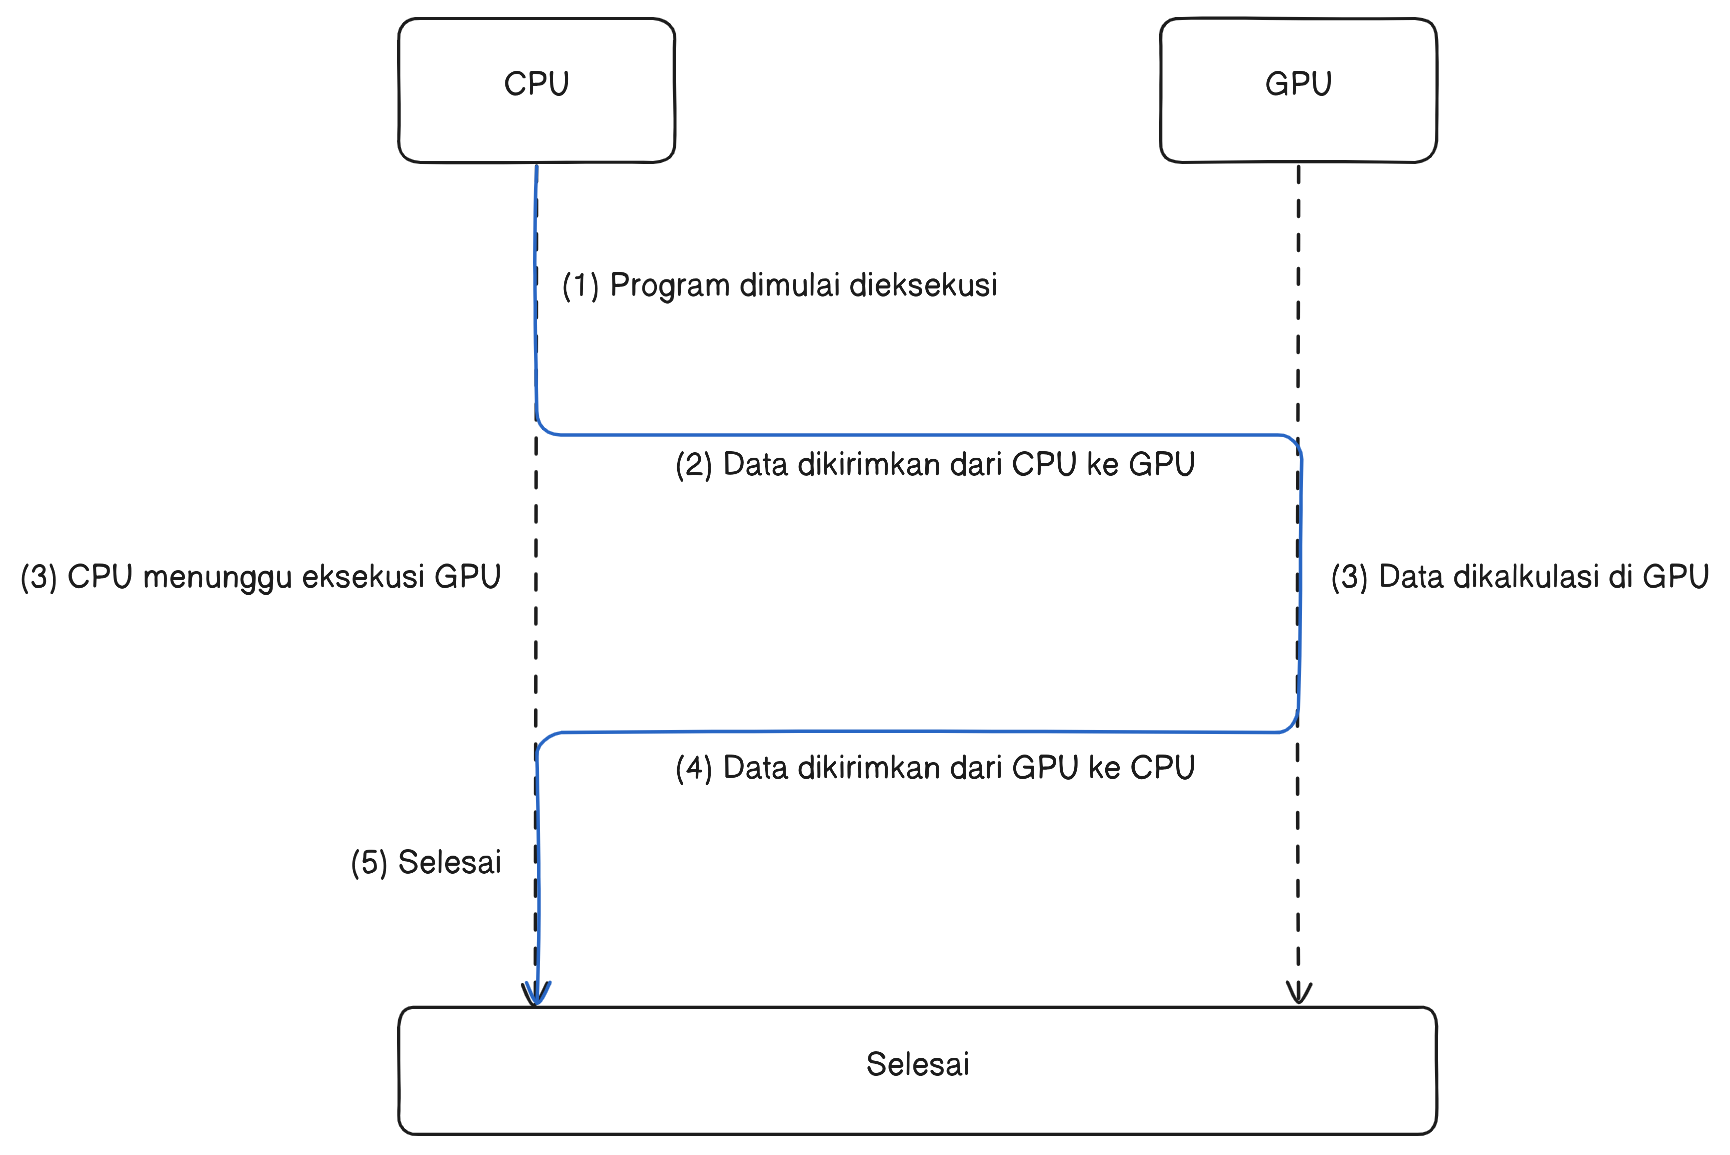
\includegraphics[width=14cm, scale=1]{images/process-cpu-gpu-calculation.png}
	\caption{Proses eksekusi program yang dikalkulasi di GPU}
	\label{img:process-cpu-gpu-calculation}
\end{figure}

Secara garis besar, proses eksekusi program yang dikalkulasi di GPU dapat digambarkan seperti yang terlihat pada Gambar \ref{img:process-cpu-gpu-calculation}. Jika menggunakan Gambar \ref{img:process-cpu-gpu-calculation} dan kode pada Lampiran \ref{appx:addition}, proses nya adalah sebagai berikut:

\begin{enumerate}
	\item CPU memulai eksekusi pada program
	\item Data dikirimkan/disalin dari CPU ke GPU dengan cara
	      \begin{lstlisting}
      # A_normal: Data di CPU
      # A: Data di GPU
      # CUDA.convert: Menyalin data A_normal (di CPU) ke data A (di GPU)
      A = CUDA.convert(CuArray{Float16}, A_normal)
      \end{lstlisting}
	\item Data dikalkulasi oleh GPU dengan cara
	      \begin{lstlisting}
	C = CUDA.zeros(Float16, size(A)) # membuat array kosong berukuran matriks A
	CUDA.@sync C .= A .+ B # mengkalkulasi matriks di GPU
      \end{lstlisting}
	      Sembari proses ini berlangsung, karena terdapat \cw{@async}, maka CPU menunggu GPU hingga proses kalkulasi selesai.
	\item GPU mengirim hasil kalkulasi ke CPU dengan menggunakan \emph{operator assignment} "\cw{=}".
	\item CPU selesai menjalankan program
\end{enumerate}

Pada penjelasan diatas, penulis menggunakan kode simulasi operasi penjumlahan pada Lampiran \ref{appx:addition}. Untuk simulasi operasi lainnya, secara garis besar mempunyai proses eksekusi yang sama seperti operasi penjumlahan. Semua kode simulasi sudah penulis lampirkan di bagian Lampiran.

\section{Validasi Hasil Simulasi}

Sebelum memasuki bagian hasil simulasi perbandingan durasi eksekusi sistem series oleh CPU dan sistem paralel oleh GPU, diperlukan validasi hasil simulasi agar dapat memastikan bahwa simulasi telah berjalan semestinya. Penulis hanya akan melakukan validasi hasil pada simulasi pencarian nilai eigen, dikarenakan pencarian nilai eigen ini merupakan satu satu nya metode yang menggunakan data elemen bukan acak, melainkan menggunakan data matriks berdasarkan Persamaan \ref{eq:schrodinger_finite_matrix}.

Dari Persamaan \ref{eq:schrodinger_finite_matrix}, akan diperoleh nilai eigen yang mana dapat dikonversi ke bentuk energi dengan menggunakan Persamaan \ref{eq:numerical_energy}, dan hasilnya dapat dibandingkan dengan Persamaan \ref{eq:analytical_energy}. Pada validasi ini penulis hanya menggunakan 3 ukuran matriks, yakni 100x100 (mewakili matriks berukuran kecil), 1000x1000 (mewakili matriks berukuran menengah), dan 9920x9920 (mewakili matriks berukuran besar). Tabel \ref{tab:result_validation_1}, Tabel \ref{tab:result_validation_2}, dan Tabel \ref{tab:result_validation_3}.

\begin{table}[H]
	\centering
	\caption{Hasil Validasi Nilai Energi pada pendekatan analitik dan numerik dengan Matriks Berukuran 100x100}
	\label{tab:result_validation_1}
	\begin{tabular}{|c|c|c|c|c|}
		\hline
		\textbf{Keadaan} & \textbf{CPU (Joule)} & \textbf{GPU (Joule)} & \textbf{Analitik (Joule)} & \textbf{Perbedaan (\%)} \\
		\hline
		1                & 1.47645e-38          & 1.47645e-38          & 1.50617e-38               & 1.97311                 \\
		2                & 5.90413e-38          & 5.90413e-38          & 6.02467e-38               & 2.00075                 \\
		3                & 1.32788e-37          & 1.32788e-37          & 1.35555e-37               & 2.04094                 \\
		4                & 2.35934e-37          & 2.35934e-37          & 2.40987e-37               & 2.09649                 \\
		5                & 3.6838e-37           & 3.6838e-37           & 3.76542e-37               & 2.16762                 \\
		6                & 5.29996e-37          & 5.29996e-37          & 5.4222e-37                & 2.25445                 \\
		7                & 7.20627e-37          & 7.20627e-37          & 7.38022e-37               & 2.35695                 \\
		8                & 9.40088e-37          & 9.40088e-37          & 9.63947e-37               & 2.47509                 \\
		9                & 1.18817e-36          & 1.18817e-36          & 1.22e-36                  & 2.60884                 \\
		10               & 1.46462e-36          & 1.46462e-36          & 1.50617e-36               & 2.75814                 \\
		\hline
	\end{tabular}
\end{table}

\begin{table}[H]
	\centering
	\caption{Hasil Validasi Nilai Energi pada pendekatan analitik dan numerik dengan Matriks Berukuran 1000x1000}
	\label{tab:result_validation_2}
	\begin{tabular}{|c|c|c|c|c|}
		\hline
		\textbf{Keadaan} & \textbf{CPU (Joule)} & \textbf{GPU (Joule)} & \textbf{Analitik (Joule)} & \textbf{Perbedaan (\%)} \\
		\hline
		1                & 1.51197e-38          & 1.51197e-38          & 1.50617e-38               & 0.385553                \\
		2                & 6.01974e-38          & 6.01974e-38          & 6.02467e-38               & 0.0817454               \\
		3                & 1.35363e-37          & 1.35363e-37          & 1.35555e-37               & 0.141764                \\
		4                & 2.40582e-37          & 2.40582e-37          & 2.40987e-37               & 0.168109                \\
		5                & 3.75862e-37          & 3.75862e-37          & 3.76542e-37               & 0.180618                \\
		6                & 5.41201e-37          & 5.41201e-37          & 5.4222e-37                & 0.187963                \\
		7                & 7.36598e-37          & 7.36598e-37          & 7.38022e-37               & 0.192921                \\
		8                & 9.62051e-37          & 9.62051e-37          & 9.63947e-37               & 0.196658                \\
		9                & 1.21756e-36          & 1.21756e-36          & 1.22e-36                  & 0.199811                \\
		10               & 1.50312e-36          & 1.50312e-36          & 1.50617e-36               & 0.202592                \\
		\hline
	\end{tabular}
\end{table}

\begin{table}[H]
	\centering
	\caption{Hasil Validasi Nilai Energi pada pendekatan analitik dan numerik dengan Matriks Berukuran 9920x9920}
	\label{tab:result_validation_3}
	\begin{tabular}{|c|c|c|c|c|}
		\hline
		\textbf{Keadaan} & \textbf{CPU (Joule)} & \textbf{GPU (Joule)} & \textbf{Analitik (Joule)} & \textbf{Perbedaan (\%)} \\
		\hline
		1                & 4.13446e-38          & 4.13446e-38          & 1.50617e-38               & 174.502                 \\
		2                & 1.0441e-37           & 1.0441e-37           & 6.02467e-38               & 73.3049                 \\
		3                & 1.57082e-37          & 1.57082e-37          & 1.35555e-37               & 15.8808                 \\
		4                & 2.95729e-37          & 2.95729e-37          & 2.40987e-37               & 22.7161                 \\
		5                & 4.51511e-37          & 4.51511e-37          & 3.76542e-37               & 19.9101                 \\
		6                & 7.20077e-37          & 7.20077e-37          & 5.4222e-37                & 32.8017                 \\
		7                & 8.57807e-37          & 8.57807e-37          & 7.38022e-37               & 16.2306                 \\
		8                & 9.8158e-37           & 9.8158e-37           & 9.63947e-37               & 7.50736                 \\
		9                & 1.38373e-36          & 1.38373e-36          & 1.22e-36                  & 13.4209                 \\
		10               & 1.58821e-36          & 1.58821e-36          & 1.50617e-36               & 5.44722                 \\
		\hline
	\end{tabular}
\end{table}

Berdasarkan Tabel \ref{tab:result_validation_1}, Tabel \ref{tab:result_validation_2}, dan Tabel \ref{tab:result_validation_3}; pendekatan metode beda hingga pada persamaan schrodinger mempunyai hasil nilai paling bagus jika menggunakan matriks yang ukuran nya menengah, yakni dengan matriks dengan kisaran ukuran 1000x1000, yang mana mempunyai perbedaan kurang dari 1\% jika dibandingkan dengan hasil analitik nya.

Berdasarkan jumlah diskritisasi, seharusnya semakin besar ukuran matriks menghasilkan peningkatan resolusi. Namun pada ukuran 9920x9920, diperoleh hasil yang menjauhi nilai analitik nya. Ini kemungkinan disebabkan karena ukuran matriks 9920x9920 merupakan ukuran dimana batas matriks bisa dijalankan oleh laptop penulis (batas maksimal 9924x9924), sehingga kemungkinan terdapat kendala yang menyebabkan nilai nya menjadi menjauhi hasil analitik nya. Kemungkinan lainnya adalah, ukuran matriks yang melebihi 1000x1000 akan menghasilkan nilai eigen yang divergensi pada pendekatan beda-hingga untuk Persamaan Schrodinger.

Hasil grafik validasi fungsi eigen dapat dilihat pada Gambar \ref{img:evaluation_1}, Gambar \ref{img:evaluation_2}, dan Gambar \ref{img:evaluation_3}, yang mana berdasarkan \cite{griffithsIntroductionQuantumMechanics2019} hasil grafik tersebut memiliki hasil yang sesuai dengan grafik fungsi eigen analitik nya.

\begin{figure}[H]
	\centering
	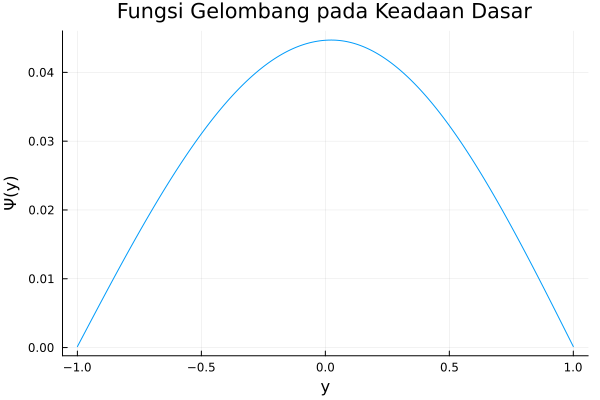
\includegraphics[width=12cm, scale=1]{images/penelitian/evaluation_1.png}
	\caption{Grafik Fungsi Eigen berdasarkan Pendekatan Numerik pada Keadaan Dasar}
	\label{img:evaluation_1}
\end{figure}

\begin{figure}[H]
	\centering
	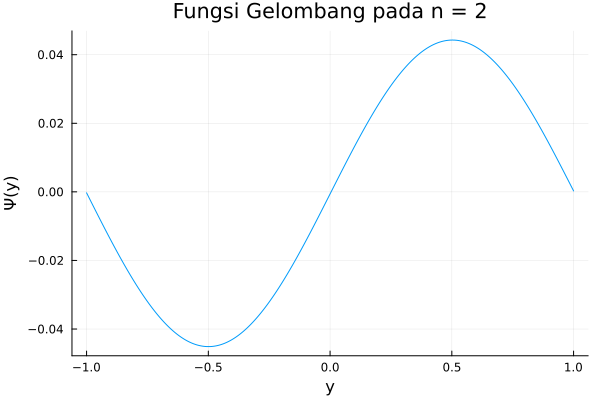
\includegraphics[width=14cm, scale=1]{images/penelitian/evaluation_2.png}
	\caption{Grafik Fungsi Eigen berdasarkan Pendekatan Numerik pada Keadaan n = 1}
	\label{img:evaluation_2}
\end{figure}

\begin{figure}[H]
	\centering
	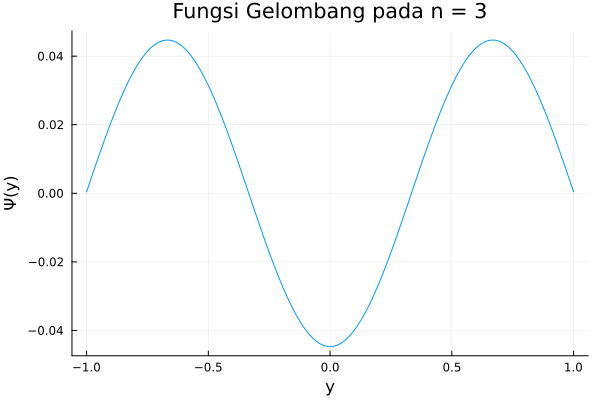
\includegraphics[width=14cm, scale=1]{images/penelitian/evaluation_3.png}
	\caption{Grafik Fungsi Eigen berdasarkan Pendekatan Numerik pada Keadaan n = 2}
	\label{img:evaluation_3}
\end{figure}

\section{Hasil Simulasi}

\subsection{Operasi Penjumlahan}

Perbandingan kecepatan eksekusi operasi penjumlahan secara series oleh CPU dan secara paralel oleh GPU menghasilkan Gambar \ref{img:result_addition}. Terlihat bahwa eksekusi series oleh CPU berhasil lebih cepat daripada eksekusi paralel oleh GPU pada ukuran matriks yang kecil. Namun, seiring bertambahnya ukuran matriks, kecepatan eksekusi paralel oleh GPU berhasil lebih cepat daripada kecepatan eksekusi series oleh CPU.

Meskipun secara grafik terlihat bahwa terdapat perbedaan kecepatan eksekusi yang signifikan, namun jika dilihat dari Tabel \ref{tab:result_addition}, semua eksekusi memerlukan waktu kurang dari 1 detik. Sehingga, operasi penjumlahan matriks masih bisa dianggap berjalan dengan baik di CPU maupun di GPU.

\begin{figure}[H]
	\centering
	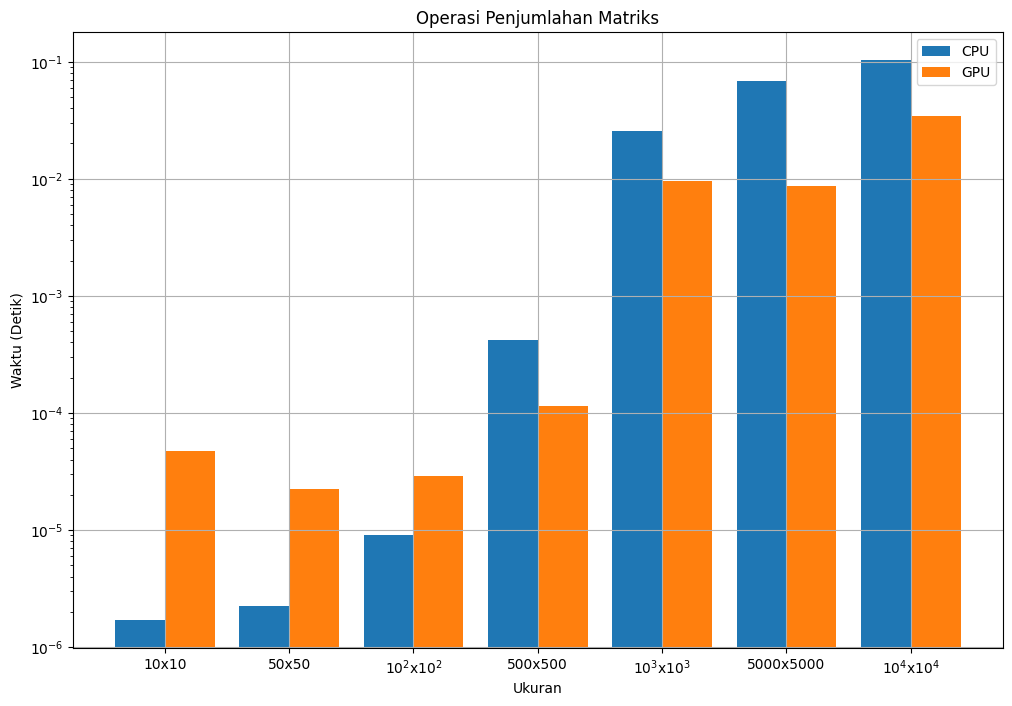
\includegraphics[width=14cm, scale=1]{images/penelitian/addition.png}
	\caption{Hasil dari Operasi Penjumlahan Matriks}
	\label{img:result_addition}
\end{figure}

\begin{table}[H]
	\centering
	\caption{Hasil dari Operasi Penjumlahan Matriks}
	\label{tab:result_addition}
	\begin{tabular}{ccc}
		\toprule
		Variasi & CPU (s)  & GPU (s)  \\
		\midrule
		1       & 0.000002 & 0.000047 \\
		2       & 0.000002 & 0.000022 \\
		3       & 0.000009 & 0.000029 \\
		4       & 0.000423 & 0.000115 \\
		5       & 0.025585 & 0.009535 \\
		6       & 0.068290 & 0.008593 \\
		7       & 0.102998 & 0.034617 \\
		\bottomrule
	\end{tabular}
\end{table}

\subsection{Operasi Pengurangan}

Berdasarkan penjelasan pada bagian \ref{Operasi Pengurangan}, operasi pengurangan merupakan modifikasi sederhana dari operasi penjumlahan. Sehingga diperkirakan akan memiliki hasil yang hampir sama dengan operasi penjumlahan. Hasil dari operasi pengurangan pada eksekusi series oleh CPU dan eksekusi paralel oleh GPU dapat dilihat pada Tabel \ref{tab:result_substraction} yang mana dapat dibentuk grafik pada Gambar \ref{img:result_substraction}.

\begin{figure}[H]
	\centering
	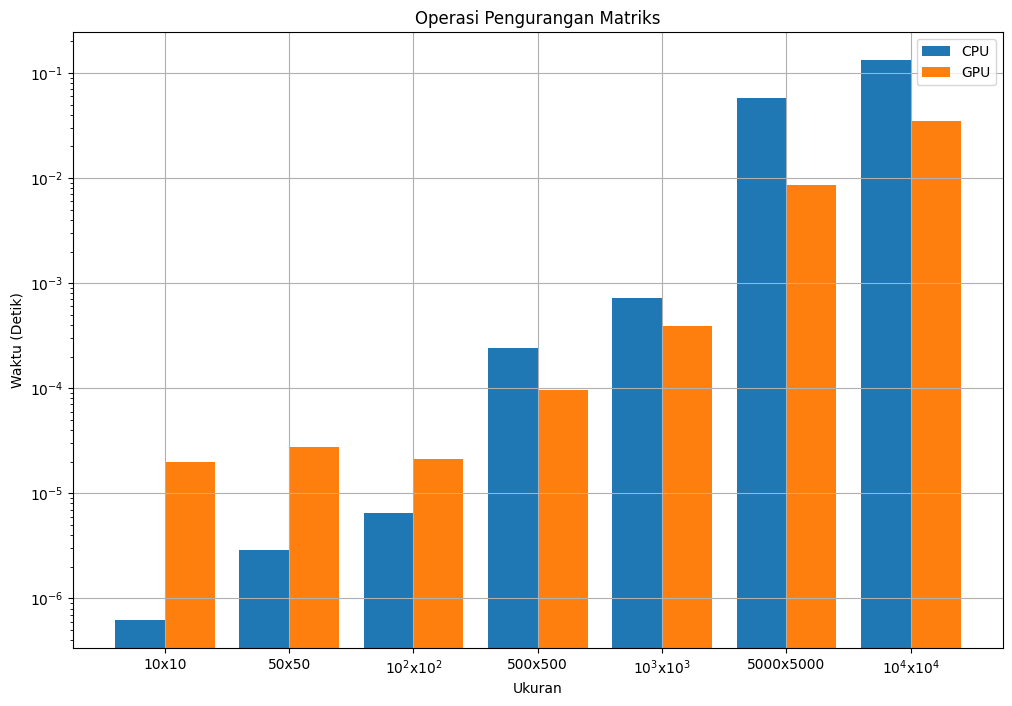
\includegraphics[width=14cm, scale=1]{images/penelitian/substraction.png}
	\caption{Hasil dari Operasi Pengurangan Matriks}
	\label{img:result_substraction}
\end{figure}

\begin{table}[H]
	\centering
	\caption{Hasil dari Operasi Pengurangan Matriks}
	\label{tab:result_substraction}
	\begin{tabular}{ccc}
		\toprule
		Variasi & CPU (s)              & GPU (s)              \\
		\midrule
		1       & $6.2 \times 10^{-7}$ & $2.0 \times 10^{-5}$ \\
		2       & $2.9 \times 10^{-6}$ & $2.8 \times 10^{-5}$ \\
		3       & $6.5 \times 10^{-6}$ & $2.1 \times 10^{-5}$ \\
		4       & $2.4 \times 10^{-4}$ & $9.6 \times 10^{-5}$ \\
		5       & $7.2 \times 10^{-4}$ & $3.9 \times 10^{-4}$ \\
		6       & $5.8 \times 10^{-2}$ & $8.6 \times 10^{-3}$ \\
		7       & $1.3 \times 10^{-1}$ & $3.5 \times 10^{-2}$ \\
		\bottomrule
	\end{tabular}
\end{table}

Berdasarkan Gambar \ref{img:result_substraction}, terlihat bahwa eksekusi series oleh CPU lebih cepat daripada eksekusi paralel oleh GPU pada matriks berukuran kecil. Seiring bertambahnya ukuran matriks, kecepatan eksekusi paralel oleh GPU berhasil lebih cepat daripada kecepatan eksekusi series oleh CPU.

Meskipun seiring bertambah nya ukuran matriks kecepatan eksekusi paralel oleh GPU lebih cepat daripada kecepatan eksekusi series oleh CPU, perbedaan antara kecepatan eksekusi yang diperoleh pada seperti yang terlihat pada Tabel \ref{tab:result_substraction}, tidak terlalu berbeda dan secara semua nya dibawah 1 detik. Untuk itu, operasi pengurangan matriks masih bisa dianggap berjalan dengan baik di CPU maupun di GPU.

\subsection{Operasi Perkalian Skalar dengan Matrik}

Berdasarkan \ref{Operasi Perkalian dengan Skalar} merupakan modifikasi yang lebih kompleks dari operasi penjumlahan. Untuk itu, diperkirakan akan diperoleh hasil yang sedikit berbeda daripada operasi penjumlahan dan operasi pengurangan. Hasil dari perkalian skalar dengan matriks pada eksekusi series oleh CPU dan eksekusi paralel oleh GPU dapat dilihat pada Tabel \ref{tab:result_scalar_matrix_multiplication} yang mana hasil tersebut dapat dibentuk grafik Gambar \ref{img:result_scalar_matrix_multiplication}.

\begin{figure}[H]
	\centering
	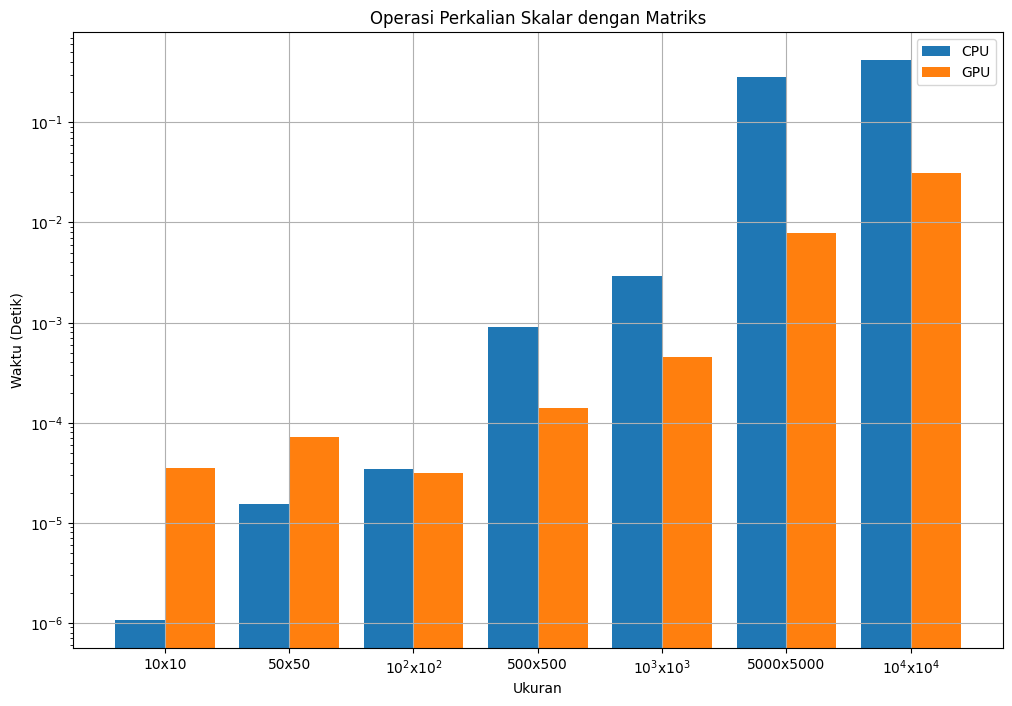
\includegraphics[width=14cm, scale=1]{images/penelitian/scalar-matrix-multiplication.png}
	\caption{Hasil dari Operasi Perkalian Skalar dengan Matriks}
	\label{img:result_scalar_matrix_multiplication}
\end{figure}

\begin{table}[H]
	\centering
	\caption{Hasil dari Operasi Perkalian Skalar dengan Matriks}
	\label{tab:result_scalar_matrix_multiplication}
	\begin{tabular}{ccc}
		\toprule
		Variasi & CPU (s)  & GPU (s)  \\
		\midrule
		1       & 0.000001 & 0.000036 \\
		2       & 0.000016 & 0.000071 \\
		3       & 0.000034 & 0.000032 \\
		4       & 0.000913 & 0.000141 \\
		5       & 0.002931 & 0.000456 \\
		6       & 0.286256 & 0.007874 \\
		7       & 0.418853 & 0.031236 \\
		\bottomrule
	\end{tabular}
\end{table}

Berdasarkan Gambar \ref{img:result_scalar_matrix_multiplication}, terlihat bahwa kecepatan eksekusi series oleh CPU lebih cepat daripada kecepatan eksekusi paralel oleh GPU pada matriks yang berukuran kecil. Namun, seiring bertambah nya ukuran matriks, diperoleh kecepatan eksekusi paralel oleh GPU lebih cepat daripada kecepatan eksekusi series oleh CPU.

Jika dilihat dari Tabel \ref{tab:result_scalar_matrix_multiplication}, meskipun terdapat perbedaan kecepatan eksekusi series oleh CPU dan eksekusi paralel oleh GPU, waktu yang diperlukan untuk menjalankan eksekusi tersebut dibawah 1 detik. Untuk itu, dapat dikatakan bahwa operasi perkalian skalar dengan matriks dapat berjalan dengan baik di GPU dan di CPU.

\subsection{Operasi Perkalian Antar Matrik}

Berdasarkan \ref{Operasi Perkalian Matriks dengan Matriks}, operasi perkalian antar matriks merupakan modifikasi operasi penjumlahan dan operasi perkalian, sehingga dapat dibilang bahwa operasi perkalian antar matriks memiliki kompleksitas yang lebih tinggi daripada operasi perkalian skalar dengan matriks. Untuk itu, diperkirakan akan diperoleh hasil yang sangat berbeda jika dibandingkan dengan operasi - operasi sebelum nya. Hasil dari operasi perkalian antar matriks ini dapat dilihat pada Tabel \ref{tab:result_matrix_matrix_multiplication} dan Gambar \ref{img:result_matrix_matrix_multiplication}.

\begin{figure}[H]
	\centering
	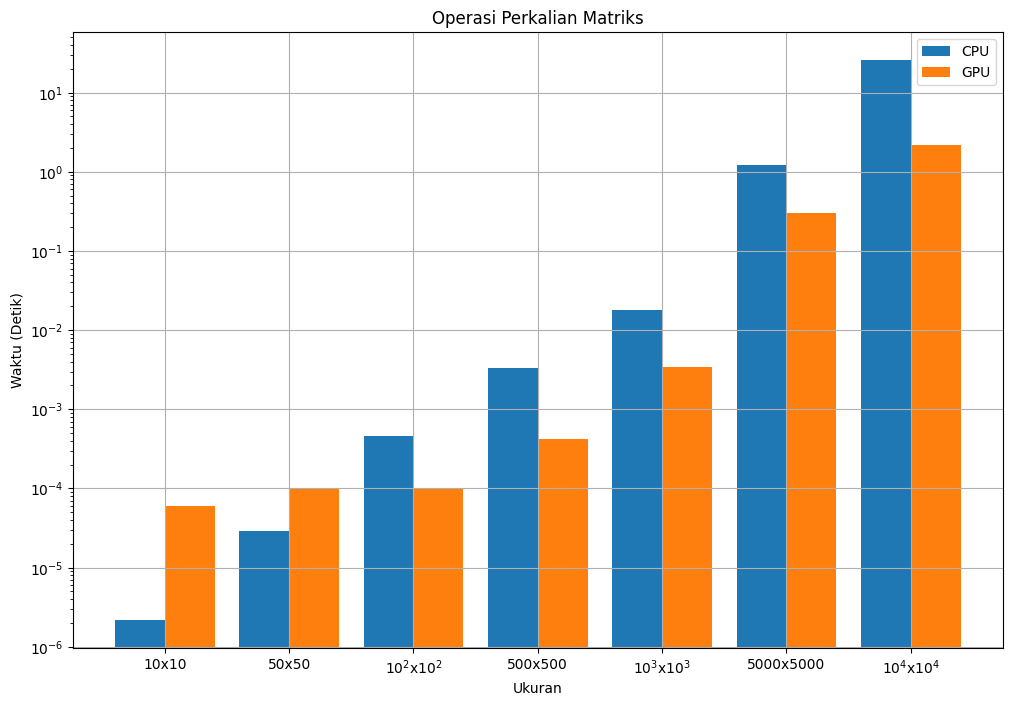
\includegraphics[width=14cm, scale=1]{images/penelitian/matrix-matrix-multiplication.png}
	\caption{Hasil dari Operasi Perkalian antar Matriks}
	\label{img:result_matrix_matrix_multiplication}
\end{figure}

\begin{table}[H]
	\centering
	\caption{Hasil dari Operasi Perkalian antar Matriks}
	\label{tab:result_matrix_matrix_multiplication}
	\begin{tabular}{ccc}
		\toprule
		Variasi & CPU (s)   & GPU (s)  \\
		\midrule
		1       & 0.000002  & 0.000060 \\
		2       & 0.000029  & 0.000097 \\
		3       & 0.000459  & 0.000098 \\
		4       & 0.003283  & 0.000416 \\
		5       & 0.017756  & 0.003405 \\
		6       & 1.231584  & 0.297797 \\
		7       & 25.754718 & 2.211518 \\
		\bottomrule
	\end{tabular}
\end{table}

Berdasarkan Gambar \ref{img:result_matrix_matrix_multiplication}, kecepatan eksekusi series oleh CPU berhasil lebih cepat daripada kecepatan eksekusi paralel oleh GPU pada matriks yang berukuran kecil. Seiring meningkatnya ukuran matriks, kecepatan eksekusi paralel oleh GPU berhasil lebih cepat daripada kecepatan eksekusi series oleh CPU.

Jika dilihat dari Tabel \ref{tab:result_matrix_matrix_multiplication}, pada variasi ke-7, kecepatan eksekusi paralel oleh GPU mempunyai durasi 2,2 detik sedangkan kecepatan eksekusi series oleh CPU mempunyai durasi 25,8 detik. Perbedaan ini cukup signifikan, dan diperkirakan akan semakin jauh perbedaannya jika ukuran matriks nya bertambah. Untuk itu, operasi perkalian antar matriks berjalan baik di CPU pada ukuran matriks yang tidak terlalu besar. Sehingga, jika terdapat operasi perkalian matriks, bisa menggunakan CPU jika ukuran matriks nya kecil, dan bisa menggunakan GPU jika ukuran matriks nya besar.

\subsection{Operasi Inverse}

Berdasarkan bagian \ref{Operasi Inverse}, operasi pencarian matriks memiliki kompleksitas yang jauh lebih tinggi daripada operasi - operasi sebelumnya. Untuk itu, diperkirakan operasi pencarian inverse matriks ini akan memperoleh hasil yang berbeda dari operasi - operasi sebelumnya. Hasil simulasi operasi inverse pada sistem series dan sistem paralel dapat dilihat pada Tabel \ref{tab:result_inverse} dan Gambar \ref{img:result_inverse}.

\begin{figure}[H]
	\centering
	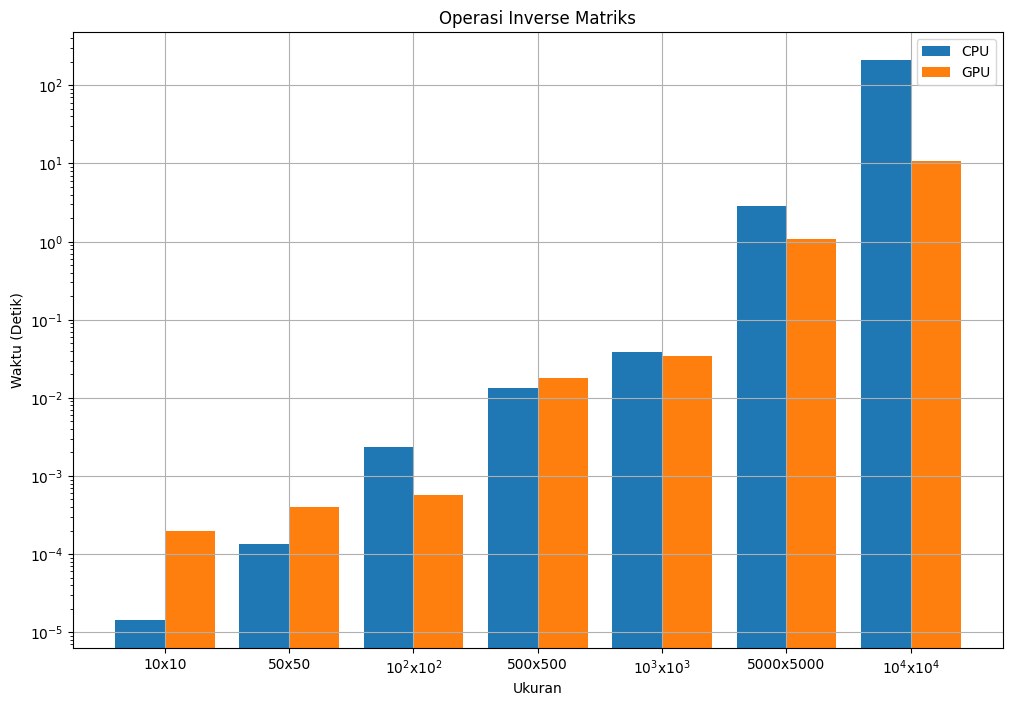
\includegraphics[width=14cm, scale=1]{images/penelitian/inverse.png}
	\caption{Hasil dari Operasi Inverse}
	\label{img:result_inverse}
\end{figure}

Berdasarkan Gambar \ref{img:result_inverse}, pada ukuran matriks yang kecil, kecepatan eksekusi series oleh CPU lebih cepat daripada kecepatan eksekusi paralel oleh GPU. Kemudian seiring meningkatnya ukuran matriks, kecepatan eksekusi paralel oleh GPU berhasil lebih cepat daripada kecepaan eksekusi series oleh CPU.

\begin{table}[H]
	\centering
	\caption{Hasil dari Operasi Inverse}
	\label{tab:result_inverse}
	\begin{tabular}{ccc}
		\toprule
		Variasi & CPU (s)    & GPU (s)   \\
		\midrule
		1       & 0.000014   & 0.000197  \\
		2       & 0.000136   & 0.000398  \\
		3       & 0.002382   & 0.000571  \\
		4       & 0.013442   & 0.017912  \\
		5       & 0.038086   & 0.034512  \\
		6       & 2.823527   & 1.068747  \\
		7       & 210.205265 & 10.711182 \\
		\bottomrule
	\end{tabular}
\end{table}

Jika dilihat dari Tabel \ref{tab:result_inverse} pada variasi ke-7, kecepatan eksekusi paralel oleh GPU mempunyai durasi kurang dari 11 detik, sedangkan kecepatan eksekusi series oleh CPU mempunyai durasi lebih dari 3 menit. Jika ukuran matriks nya ditambahkan, diperkirakan akan semakin jauh durasi ekeskusi paralel oleh GPU dan durasi eksekusi series oleh CPU. Untuk itu, jika terdapat operasi pencarian inverse matriks, bisa menggunakan CPU untuk ukuran matriks yang kecil, dan bisa menggunakan GPU untuk ukuran matriks yang besar.

% \subsection{Pencarian Nilai Eigen}
%
% Berdasarkan bagian \ref{Nilai Eigen}, operasi pencarian nilai eigen matriks merpakan operasi yang paling kompleks pada kajian ini. Untuk itu, diperkirakan hasil yang diperoleh akan berbeda dari operasi operasi sebelumnya. Hasil dari simulasi operasi pencarian nilai eigen dapat dilihat pada Tabel \ref{tab:result_eigenvalue} dan Gambar \ref{img:result_eigenvalue}.
%
% \begin{figure}[H]
% 	\centering
% 	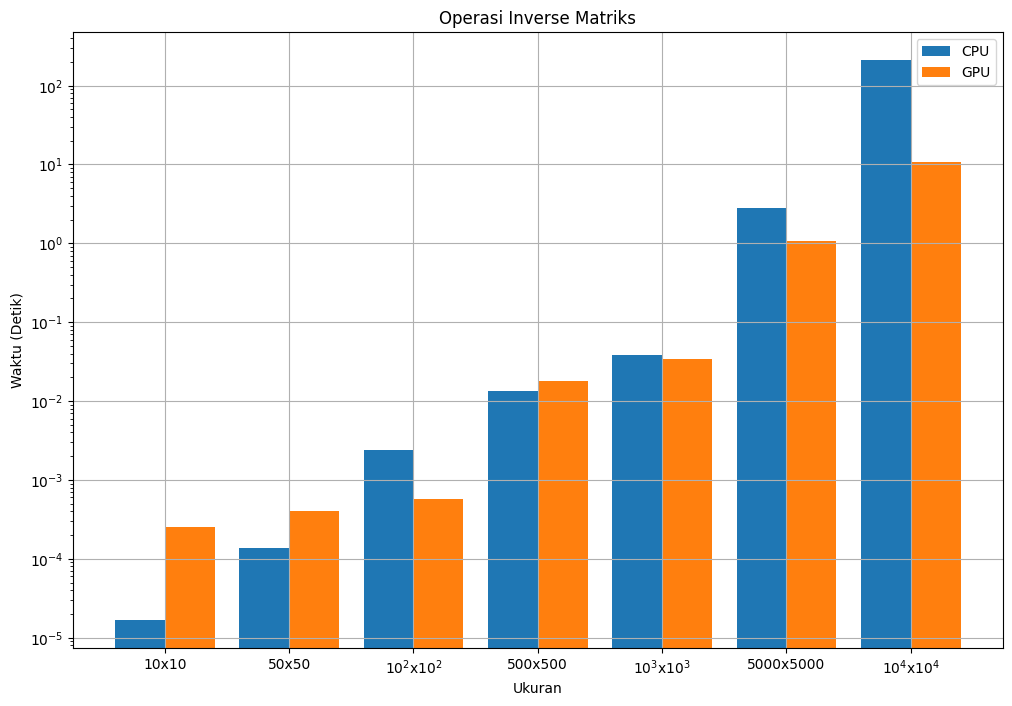
\includegraphics[width=14cm, scale=1]{images/penelitian/eigenvalue.png}
% 	\caption{Hasil dari Pencarian Nilai Eigen}
% 	\label{img:result_eigenvalue}
% \end{figure}
%
% Berdasarkan Gambar \ref{img:result_eigenvalue}, pada ukuran matriks yang kecil, kecepatan eksekusi series oleh CPU lebih cepat daripada kecepatan eksekusi paralel oleh GPU. Namun, seiring bertambahnya ukuran matriks, kecepatan eksekusi paralel oleh GPU berhasil lebih cepat daripada kecepatan eksekusi series oleh CPU.
%
% \begin{table}[H]
% 	\centering
% 	\caption{Hasil dari Pencarian Nilai Eigen}
% 	\label{tab:result_eigenvalue}
% 	\begin{tabular}{ccc}
% 		\toprule
% 		Variasi & CPU (s)    & GPU (s)   \\
% 		\midrule
% 		1       & 0.000035   & 0.000188  \\
% 		2       & 0.000718   & 0.000885  \\
% 		3       & 0.007700   & 0.001865  \\
% 		4       & 0.200065   & 0.027872  \\
% 		5       & 0.731179   & 0.121742  \\
% 		6       & 65.235088  & 5.941858  \\
% 		7       & 403.052508 & 42.954285 \\
% 		\bottomrule
% 	\end{tabular}
% \end{table}
%
% Jika dilihat dari \ref{tab:result_eigenvalue} pada variasi ke-7, kecepatan eksekusi paralel oleh GPU mempunyai durasi rata-rata kurang dari 43 detik, sedangkan kecepatan eksekusi series oleh CPU mempunyai durasi rata-rata lebih dari 6 menit. Jika ukuran matriks nya ditambah, maka diperkirakan akan menghasilkan perbedaan kecepatan yang jauh lebih berbeda antara eksekusi series oleh CPU dan eksekusi paralel oleh GPU. Untuk itu, jika terdapat operasi pencarian nilai eigen dari suatu matriks, dapat menggunakan CPU untuk ukuran matriks yang kecil, dan dapat menggunakan GPU untuk ukuran matriks yang besar.

\subsection{Operasi Pencarian Nilai Eigen}

Simulasi operasi penjumlahan hingga simulasi operasi inverse, penulis menggunakan matriks yang berisikan elemen yang bernilai acak. Pada operasi pencarian nilai eigen ini, digunakan bentuk matriks yang elemen nya bernilai tidak acak, yakni didasarkan ungkapan persamaan schrodinger melalui pendekatan metode beda-hingga pada Persamaan \ref{eq:schrodinger_finite_matrix}. Hasil dari simulasi operasi pencarian nilai eigen dapat dilihat pada Tabel \ref{tab:result_eigenvalue_schrodinger} dan Gambar \ref{img:result_eigenvalue_schrodinger}.

\begin{figure}[H]
	\centering
	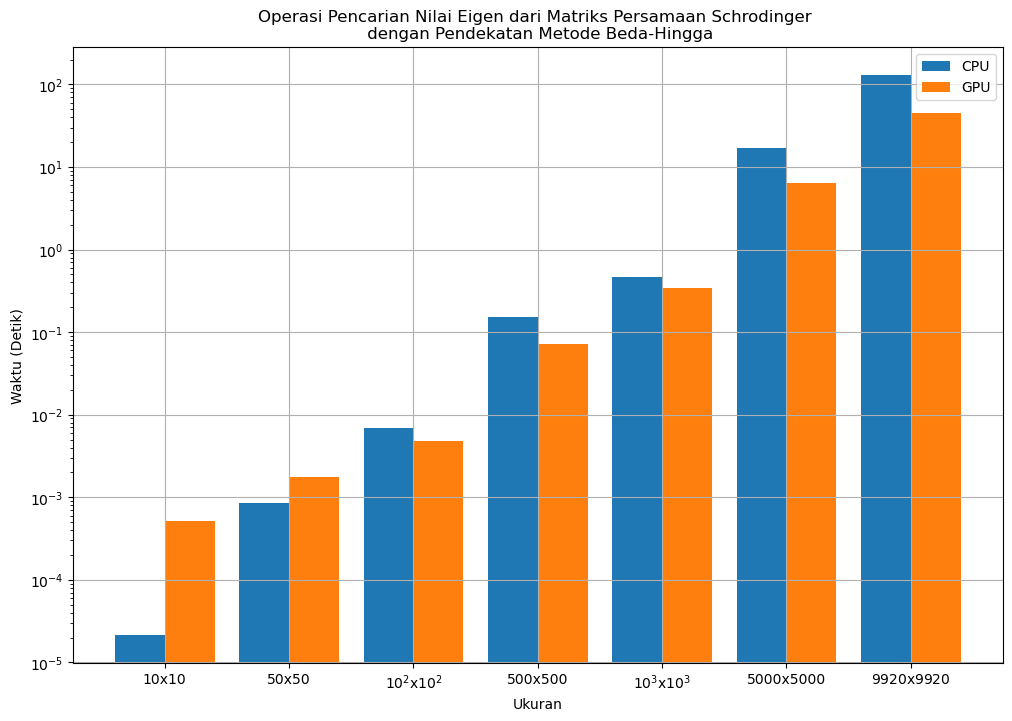
\includegraphics[width=14cm, scale=1]{images/penelitian/eigenvalue-schrodinger.png}
	\caption{Hasil dari Pencarian Nilai Eigen}
	\label{img:result_eigenvalue_schrodinger}
\end{figure}

\begin{table}[H]
	\centering
	\caption{Hasil dari Pencarian Nilai Eigen}
	\label{tab:result_eigenvalue_schrodinger}
	\begin{tabular}{ccc}
		\toprule
		Variasi & CPU (s)   & GPU (s)  \\
		\midrule
		1       & 0.000021  & 0.000514 \\
		2       & 0.000851  & 0.001738 \\
		3       & 0.006942  & 0.004741 \\
		4       & 0.151598  & 0.071691 \\
		5       & 0.466806  & 0.337955 \\
		6       & 16.79000  & 6.32500  \\
		7       & 129.82300 & 45.02900 \\
		8       & 132.49300 & 49.32900 \\
		9       & 133.11500 & 50.26700 \\
		10      & 133.79200 & 50.26700 \\
		11      & 132.51000 & 49.39700 \\
		\bottomrule
	\end{tabular}
\end{table}

Berdasarkan Gambar \ref{img:result_eigenvalue_schrodinger}, pada ukuran matriks yang kecil diperoleh keceaptan eksekusi series oleh CPU yang lebih cepat daripada kecepatan eksekusi paralel oleh GPU. Kemudian, seiring bertambahnya ukuran matriks, diperoleh kecepatan eksekusi paralel oleh GPU yang lebih cepat daripada kecepatan eksekusi series oleh CPU.

Berdasarkan Tabel \ref{tab:result_eigenvalue_schrodinger}, durasi eksekusi series oleh CPU dan kecepatan eksekusi paralel oleh GPU mempunyai nilai yang hampir sama. Pada variasi ke ke-6, kecepatan eksekusi series oleh CPU mempunyai nilai yang kurang lebih $2,65$ kali lebih lambat daripada kecepatan eksekusi paralel oleh GPU. Sedangkan pada variasi ke ke-7, kecepatan eksekusi series oleh CPU mempunyai nilai yang kurang lebih $2,88$ kali lebih lambat daripada kecepatan eksekusi paralel oleh GPU. Kemudian pada variasi ke-8 hingga ke-11, diperoleh durasi eksekusi yang hampir sama antar variasi. Pada umumnya, Julia akan menggunakan \emph{Divide-and-Conquer} atau \emph{Metode Tridiagonal QR} pada matriks simetris. Kompleksitas kedua metode tersebut adalah $\mathcal{O}(n^3)$, sehingga perbedaan ukuran matriks yang kecil tidak akan terlalu mempengaruhi kecepatan durasi eksekusi sistem series dan sistem paralel.

Perbedaan durasi eksekusi antara sistem series dan sistem paralel yang tidak terlalu besar diperkirakan karena sebagian besar Persamaan \ref{eq:schrodinger_finite_matrix} mempunyai elemen matriks yang bernilai nol, sehingga kecepatan eksekusi sistem series oleh CPU dapat mengeksekusi operasi dengan cepat. Namun, jika matriks diperbesar lagi, kemungkinan akan diperoleh perbedaan yang durasi eksekusi yang lebih jauh lagi antara eksekusi series oleh CPU dan eksekusi paralel oleh GPU.

\section{Pembahasan Secara Umum}

Pada kajian ini, dilakukan simulasi operasi matriks yang dijalankan pada sistem series oleh CPU dan sistem paralel oleh GPU. Simulasi ini dilakukan dari operasi sederhana hingga operasi yang kompleks. Eksekusi sistem series oleh CPU secara umum dapat menjalankan operasi matriks secara cepat pada matriks berukuran kecil dan pada operasi matriks yang tidak kompleks. Sedangkan eksekusi sistem paralel oleh GPU secara umum mampu menjalankan operasi matriks secara cepat pada matriks berukuran besar dan pada operasi matriks yang lebih kompleks.

Jika dilihat dari hasil gambar grafik pada masing-masing simulasi, terdapat titik dimana kecepatan eksekusi sistem paralel oleh GPU \textbf{mulai} lebih cepat daripada kecepatan eksekusi sistem series oleh CPU. Titik ini penulis sebut dengan \emph{titik balik}. Pada operasi penjumlahan, pengurangan, dan perkalian skalar dengan matriks, titik balik nya adalah di ukuran matriks $500 \times 500$ atau pada variasi ke-4. Kemudian pada operasi yang lebih kompleks, yakni operasi perkalian antar matriks, pencarian inverse, dan pencarian nilai eigen, titik balik nya ada pada ukuran matriks $100 \times 100$ atau variasi ke-3. Hasil ini dapat disimpulkan bahwa seiring meningkatnya kompleksistas operasi, eksekusi menggunakan sistem paralel oleh GPU dapat lebih efektif daripada eksekusi pada sistem series oleh CPU.

Jika dilihat dari hasil tabel pada masing-masing simulasi, semakin tinggi kompleksitas operasi maka semakin tinggi pula perbedaan durasi eksekusi pada ukuran matriks terbesar (variasi ke-7). Pada operasi penjumlahan, pengurangan, dan perkalian skalar dengan matriks, perbedaan durasi eksekusi pada variasi ke-7 secara umum mempunyai rata-rata kurang dari 1 detik. Namun, pada operasi yang lebih kompleks, yakni operasi perkalian antar matriks, pencarian inverse, dan pencarian nilai eigen, durasi eksekusi pada variasi ke-7 antara sistem series oleh CPU dan sistem paralel oleh GPU semua nya diatas 1 detik dan perbedaan paling besar ada pada simulasi operasi inverse. Dari hasil ini dapat disimpulkan bahwa seiring meningkatnya kompleksitas operasi dan seiring meningkatnya ukuran matriks, eksekusi paralel oleh GPU jauh lebih efektif daripada eksekusi series oleh CPU.

Operasi matriks tidak bergantung satu sama lain, sehingga dapat dijalankan dengan baik pada sistem paralel. Namun, dari hasil percobaan yang telah diperoleh, pada matriks berukuran kecil, sistem series lebih cepat melakukan dalam menjalankan eksekusi daripada sistem paralel. Hal ini disebabkan karena semua program pada dasarnya dijalankan di CPU. Untuk sistem series, maka eksekusi program tersebut dapat langsung dijalankan. Akan tetapi, untuk sistem paralel, eksekusi program tersebut perlu dikirimkan dari CPU ke GPU, kemudian setelah selesai dikomputasikan akan dikirimkan kembali ke CPU. Proses transfer data ini akan tampak lama jika data yang ditransferkan berukuran kecil. Dengan kata lain, proses transfer data dari CPU ke GPU dan dari GPU ke CPU akan tampak lama jika ukuran data matriks nya sedikit (matriks berukuran kecil).

Dari hasil yang telah diperoleh pada masing-masing simulasi, terlihat bahwa pada ukuran matriks yang sedikit, eksekusi sistem series oleh CPU mampu lebih cepat daripada eksekusi sistem series oleh GPU. Penulis tidak memperkirakan jika CPU dapat berjalan secepat itu. Kemungkinan cepat nya eksekusi pada CPU ini disebabkan karena CPU yang penulis pakai menggunakan Intel Core i7 tipe U generasi 10, yang mana merupakan salah satu CPU tercepat di kelas nya. Untuk itu, jika simulasi dilakukan dengan menggunakan CPU lain yang lebih lambat, diperkirakan akan diperoleh \emph{titik balik} yang lebih awal.

% Secara umum, dari setiap simulasi operasi diperoleh hasil yang sejalan dengan 

% \section{Hasil dari Metode Gauss-Seidel}
% Untuk menghitung seluruh data menggunakan program ini, dilakukan pembagian kloter yang setiap kloternya menghitung 2000--2200 data. Hal ini dilakukan untuk menghindari perhitungan yang terlalu lama, penggunaan memori yang terlalu besar, dan juga untuk mengantisipasi kesalahan yang besar. Untuk 20200, data dibagi menjadi 10 kloter perhitungan. Pada Gambar \ref{grafik_durasi} disajikan data dari 5 perhitungan waktu program. Dari data tersebut dapat kita simpulkan bahwa rata-rata waktu perhitungan untuk 2000--2200 data adalah 6712 detik atau 1,8 jam. Sehingga, untuk menghasilkan perhitungan $\phi$ untuk satu medan adalah sebesar 3,356 detik.
%
% Dalam perhitungan dengan jumlah yang besar atau simulasi kontinyu, misalnya, waktu perhitungan merupakan sesuatu yang sangat berpengaruh. Waktu 3,356 detik untuk sekitar 2000 medan akan memakan waktu yang relatif lama. Metode iteratif Gauss-Seidel memang membutuhkan waktu konvergen yang lama, namun dibandingkan dengan metode iteratif lainnya seperti Jacobi, metode Gauss-Seidel memiliki keakuratan yang relatif lebih tinggi \citep{Ford2015}. Metode Gauss-Seidel juga merupakan metode yang memberikan perkenalan mengenai konsep penggunaan iterasi untuk penyelesaian sistem (linear, dan sebagainya) dan basis untuk metode yang lebih canggih\defcitealias{Ford2015}{ibid} \citepalias{Ford2015}. Hal ini sangat baik untuk pembelajaran mahasiswa sarjana karena mudah diphami dan mudah untuk diimplementasikan.
% \begin{figure}[h!]
%     \centering
%     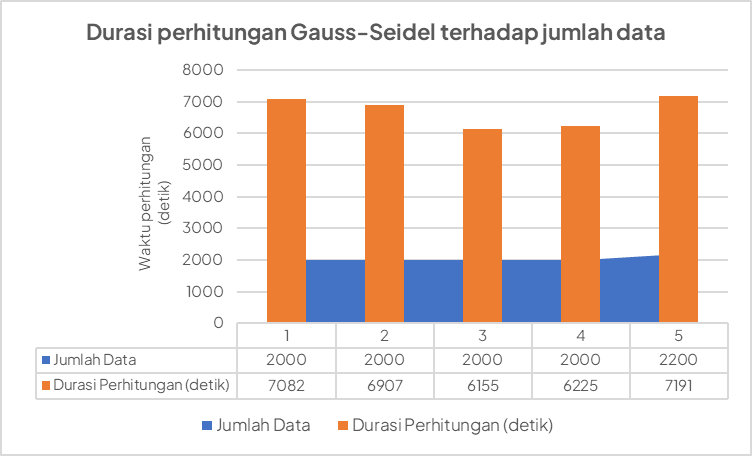
\includegraphics[width=12cm]{gambar/grafik_durasi.png}
%     \caption{Grafik durasi perhitungan Gauss-Seidel terhadap jumlah data}
%     \label{grafik_durasi}
% \end{figure}
%
% Perhitungan tersebut menghasilkan kumpulan data $\phi$ sejumlah banyaknya data $\rho$ yang memiliki rentang nilai data dari 1814160 sampai -1794090. Apabila dibandingkan dengan nilai toleransi sebesar 0,01, nilai ekstrim dari $\phi$ yang dihasilkan oleh \textit{solver} ini  relatif sangat besar, sehingga ralat yang terjadi sangat dapat diterima. Dari histogram pada Gambar \ref{hist_rata2phi} dapat kita ketahui bahwa nilai rata-rata dari $\phi$ tersebar pada rentang yang sangat besar dan relatif jauh dari nilai toleransi 0,01. Data ini tetap dapat menjustifikasi bahwa nilai toleransi ralat 0,01 merupakan nilai yang relatif sangat kecil bagi hasil $\phi$. Pesebaran nilai ekstrim dari seluruh medan terdapat pada Gambar \ref{phi_gs_rendah_tinggi}.
% \begin{figure}[h!]
%     \centering
%     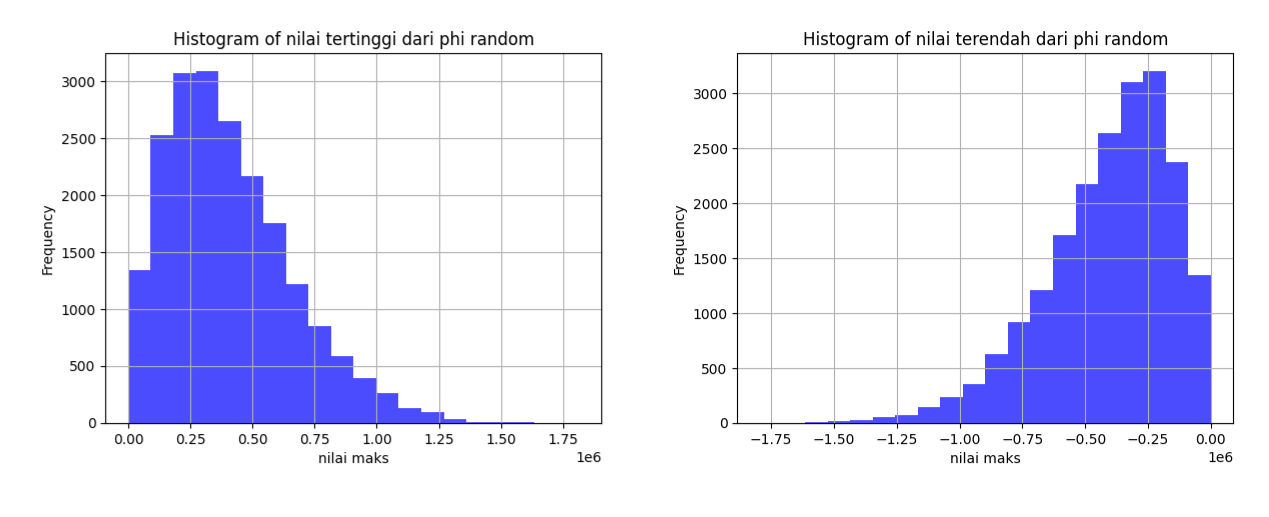
\includegraphics[width=12cm]{gambar/phi_gs_rendah_tinggi.png}
%     \caption{Kiri: Histogram nilai tertinggi pada 20200 data $\phi$. Kanan: Histogram nilai tertinggi pada 20200 data $\phi$.}
%     \label{phi_gs_rendah_tinggi}
% \end{figure}
%
% \begin{figure}[h!]
%     \centering
%     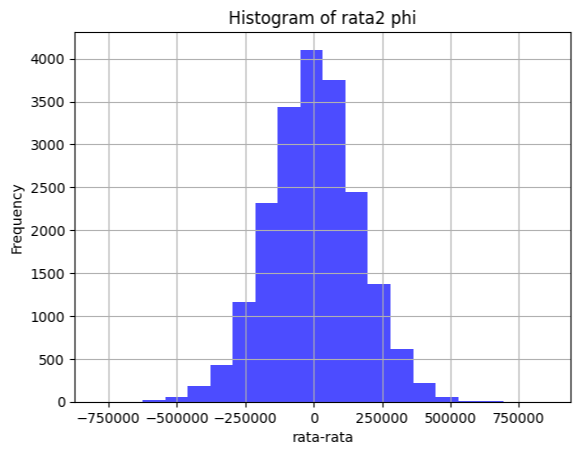
\includegraphics[width=12cm]{gambar/hist_rata2phi.png}
%     \caption{Histogram nilai rata-rata phi dari seluruh medan.}
%     \label{hist_rata2phi}
% \end{figure}
%
% \cite{cheng_illarramendi_bauerheim_cuenot_2021} menjelaskan bahwa dua puncak Gaussian yang terlihat pada medan distribusi muatan akan tersebar dan menyatu pada medan potensial yang dihasilkan. Hal ini disebutkan oleh mereka karena filter \textit{low-pass} oleh operator Laplacian terbalik. Hal yang sama dapat dilihat pada potensial yang dihasilkan dalam perhitungan ini pada Gambar \ref{rho_phi_GS}.
%
% \begin{figure}[h!]
%     \centering
%     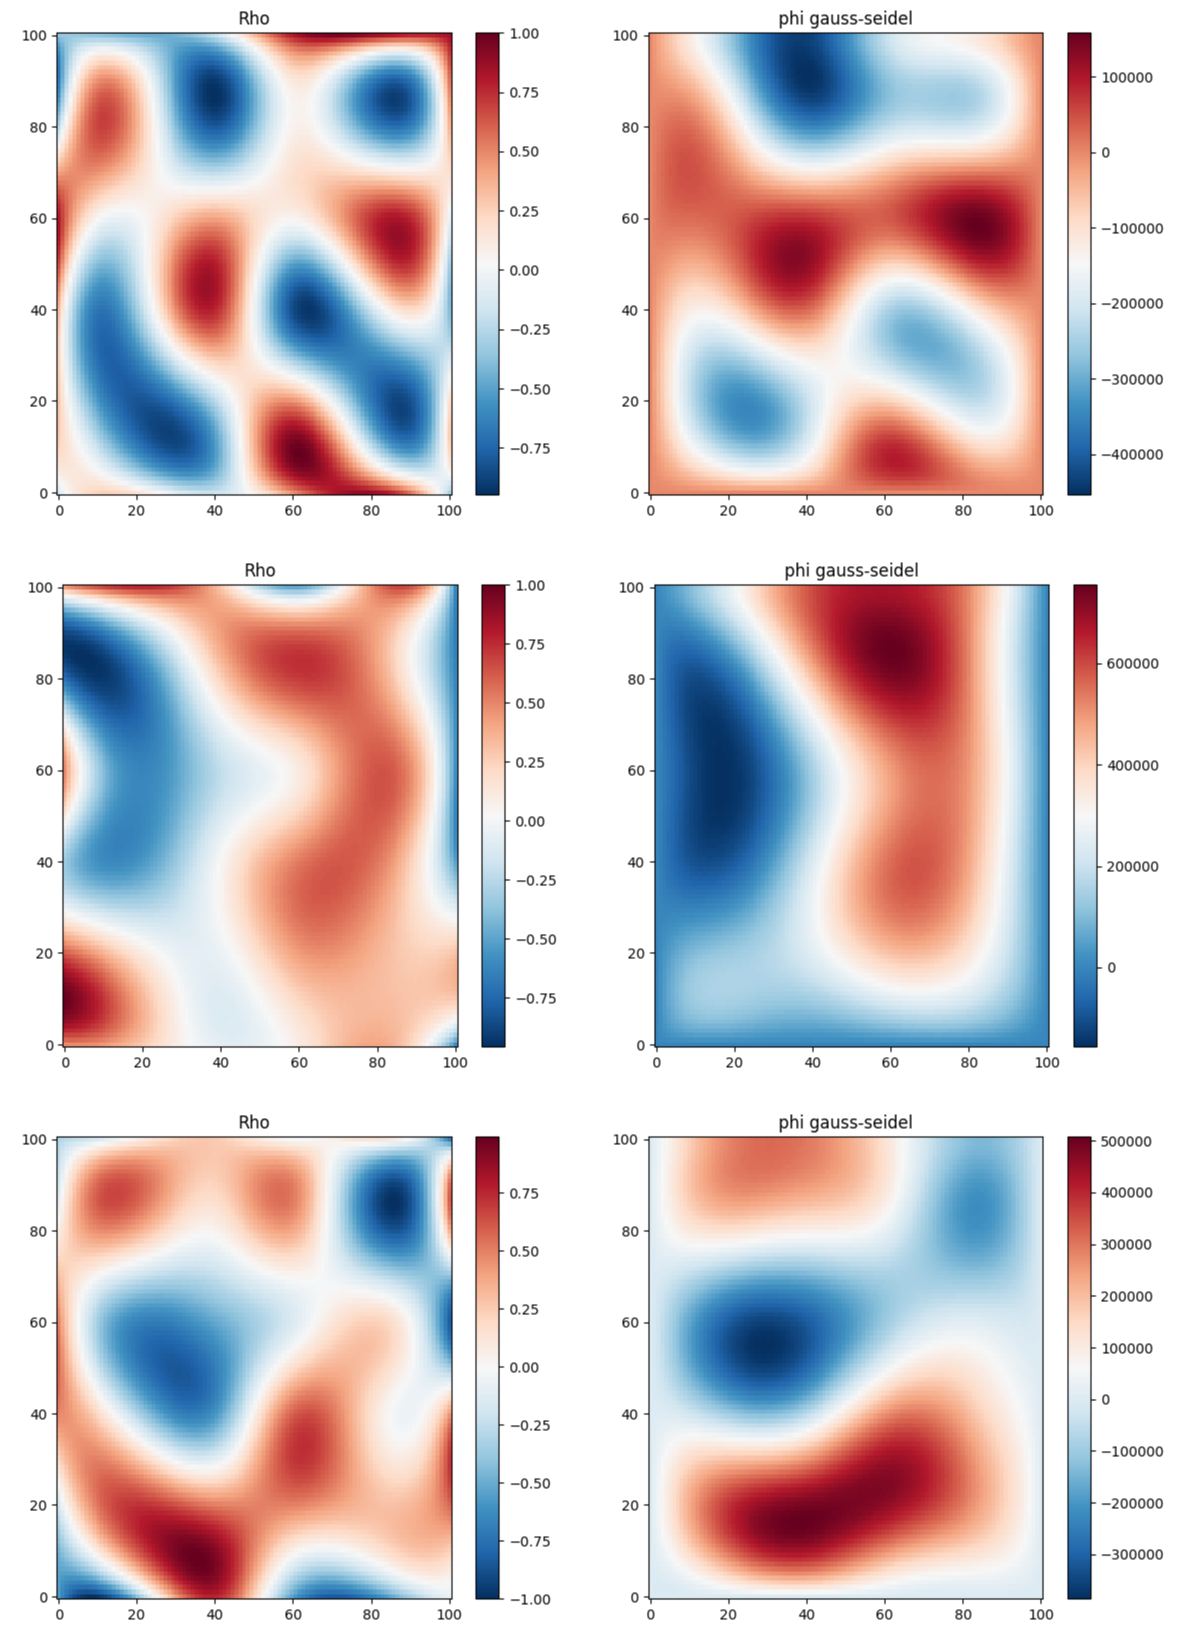
\includegraphics[width=12cm]{gambar/rho_phi_GS.png}
%     \caption{Contoh 3 pasang medan $\rho$ dan $\phi$ hasil perhitungan Gauss-Seidel}
%     \label{rho_phi_GS}
% \end{figure}
%
% Selanjutnya, data $\phi$ yang sudah terbentuk dilakukan normalisasi untuk mendapatkan skala yang sama pada tiap medan agar jaringan saraf (\textit{neural network}) dapat belajar dengan baik \citep{cheng_illarramendi_bauerheim_cuenot_2021}. Teknik penskalaan yang digunakan adalah dengan membagi keseluruhan 20200 data dengan nilai ekstrim mutlak dari keseluruhan data, dalam hal ini adalah 1814160. Setelah dilakukan normalisir, tidak terjadi perubahan distribusi pada $\phi$, hanya nilainya saja yang berubah dengan rasio 1/1814160 (Gambar \ref{rho_phi_GS_1814160}.
%
% \begin{figure}[h!]
%     \centering
%     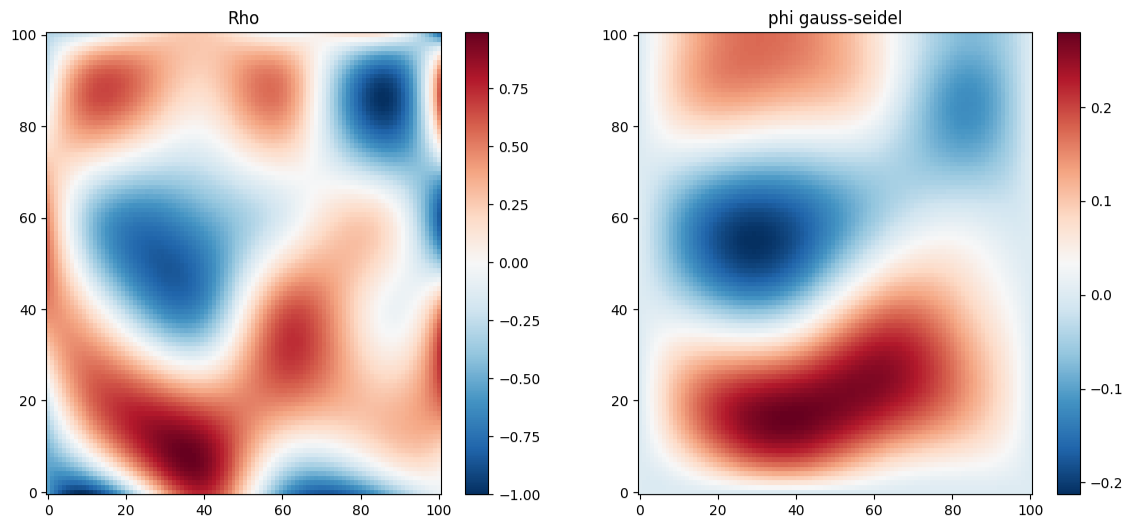
\includegraphics[width=12cm]{gambar/rho_phi_GS_1814160.png}
%     \caption{Gambar ke-3 dari Gambar \ref{rho_phi_GS} yang sudah dinormalisir dengan cara dibagi dengan 1814160.}
%     \label{rho_phi_GS_1814160}
% \end{figure}
%
% \section{Pelatihan Jaringan Saraf \textit{Neural Network}}
%
% \subsection{Arsitektur U-Net}
% Arsitektur yang digunakan pada penelitian ini adalah U-Net (Subbagian \ref{sub_unet}) yang terlampir pada Lampiran \ref{unies_og}. Penggambaran grafis mengenai arsitektur yang digunakan digambarkan pada Gambar \ref{arsitektur_unies}.
%
% \begin{figure}[h!]
%     \centering
%     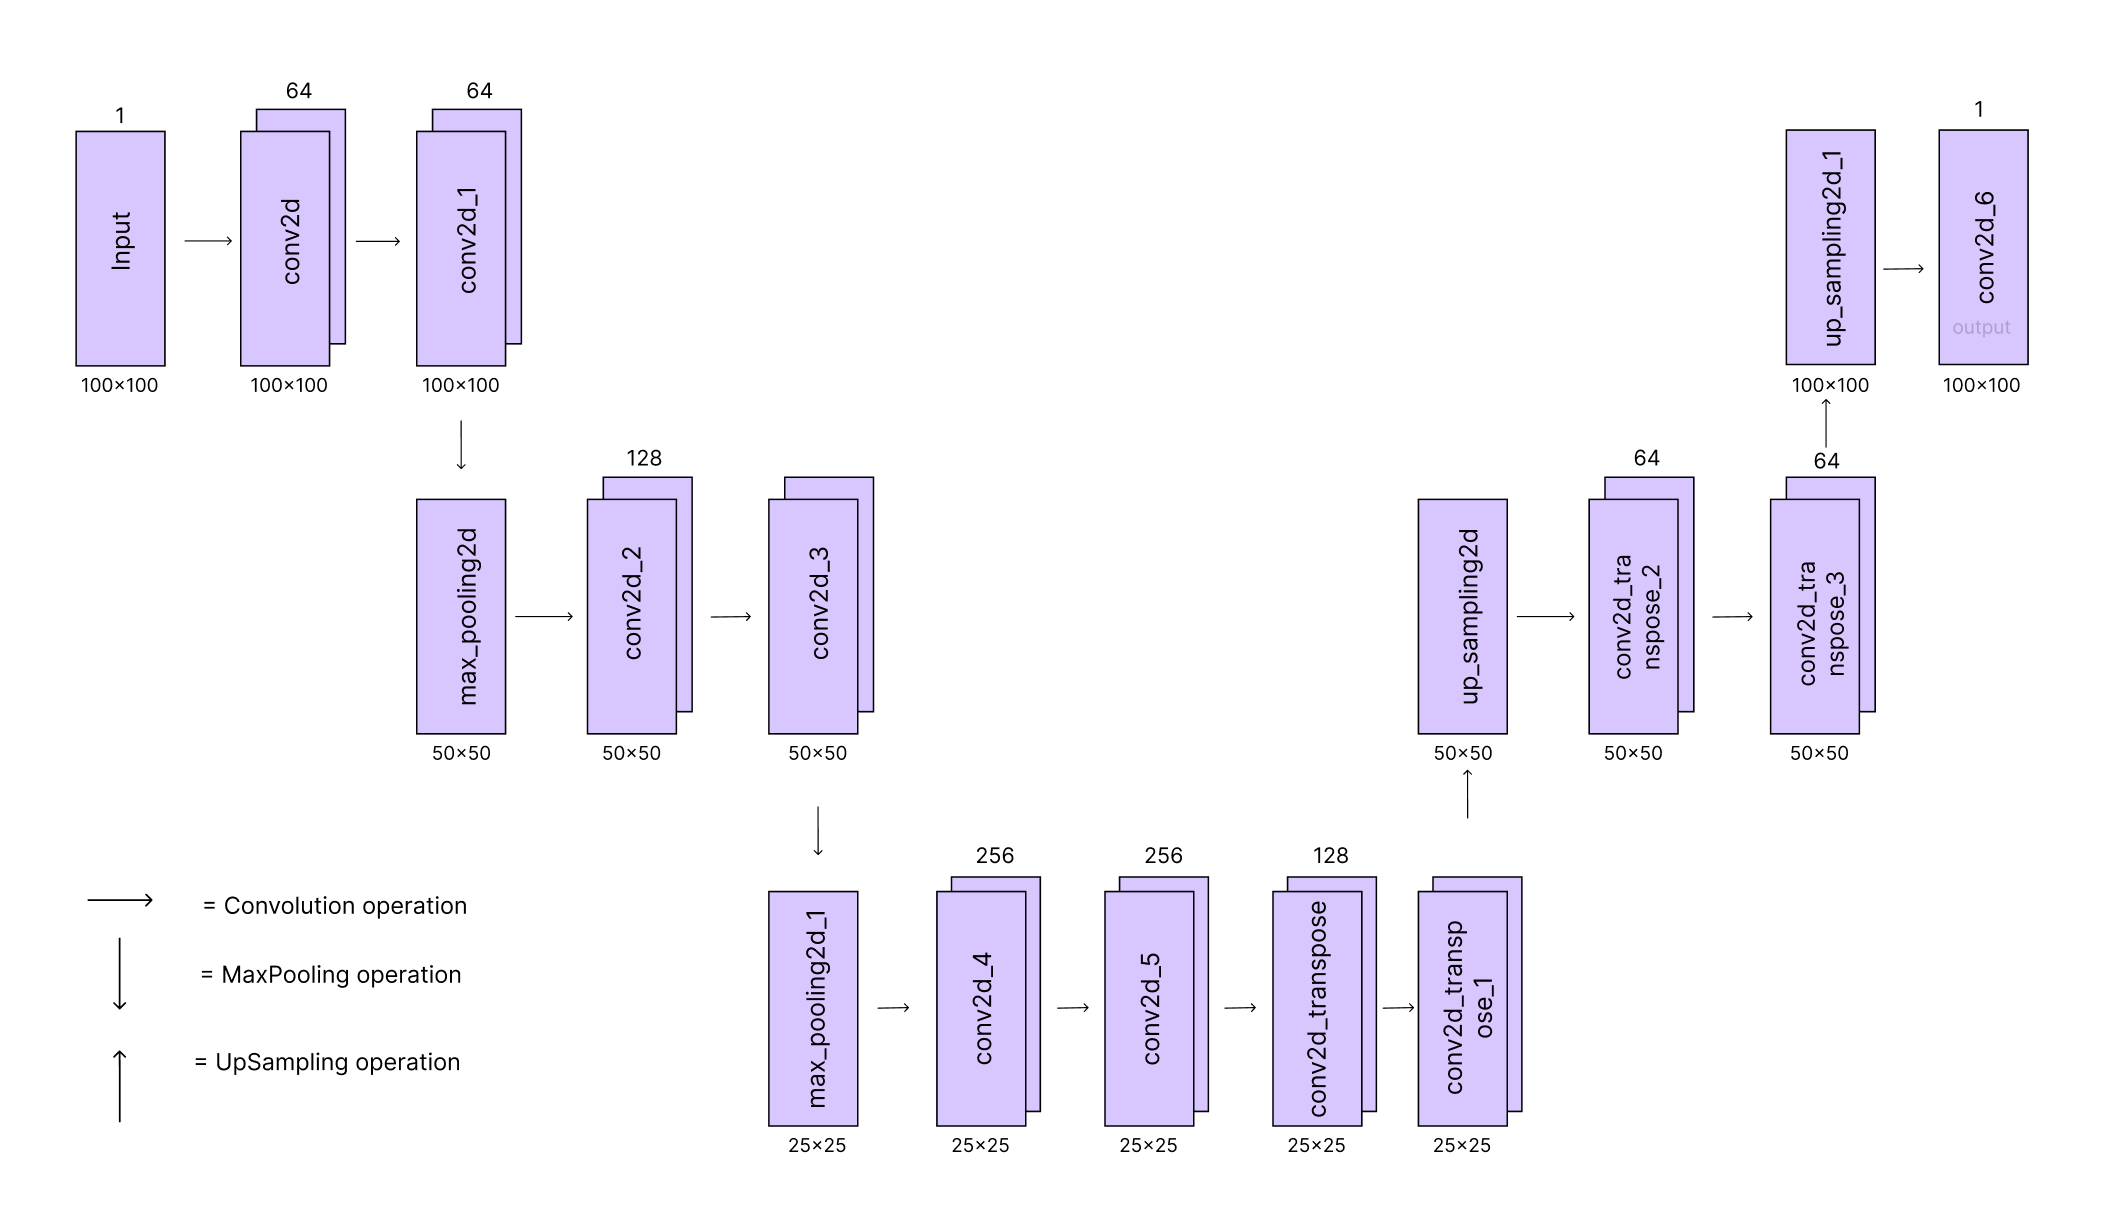
\includegraphics[width=14cm]{gambar/unies_og.png}
%     \caption{Grafik arsitektur yang digunakan. Angka di atas filter adalah jumlah filter yang digunakan, dan angka di bawah filter merupakan ukuran filter yang digunakan.}
%     \label{arsitektur_unies}
% \end{figure}
%
% Ukuran filter atau medan penerimaan (\textit{receptive field}) serta jumlah filter yang digunakan adalah bagian dari penelitian yang mencoba-coba hingga didapatkan hasil terbaik sesuai yang diharapkan. Untuk bentuk arsitektur, tidak seperti U-Net yang awalnya dicetuskan oleh \cite{DBLP:journals/corr/RonnebergerFB15}, ada modifikasi pada bagian \textit{crop and copy} yang berfungsi untuk membuang dan menyalin bagian tepi dari medan \citep{siddique_paheding_elkin_devabhaktuni_2021}. Hal ini sesuai dengan percobaan yang dilakukan \cite{alom2018recurrent} yang memodifikasi U-Net menjadi \textit{Recurrent U-Net} (RU-Net) yang menghasilkan arsitektur yang lebih mutakhir dan memiliki peforma yang lebih baik.
%
% \subsection{Pelatihan}
%
% Pelatihan dilakukan menggunakan Google Colab Pro dengan menggunakan GPU T4. Untuk melatih 1.698.177 parameter dengan 200 \textit{epoch}, dibutuhkan waktu 2 jam 30 menit (45 detik per \textit{epoch}). Untuk mengevaluasi model, dibutuhkan sampel data validasi yang dapat digunakan untuk memberikan evaluasi kesesuaian model yang tidak bias pada set data pelatihan sambil menyetel \textit{hyperparameter} model \citep{elgendy_2020}. Set data validasi yang digunakan pada pelatihan ini menggunakan 25\% dari total set data latih (5050 data).
%
% Dalam rangka mengupayakan agar model jaringan saraf atau algoritma pembelajaran dapat berkembang atau lebih cepat beradaptasi pada bobot model terhadap set data latih, maka dilakukan konfigurasi laju pemelajaran (\textit{learning rate}). Laju pemelajaran dapat dikatakan sebagai jumlah perubahan pada model selama setiap langkah proses pencarian solusi (titik optimal global), atau bisa disebut juga sebagai ukuran langkah \citep{brownlee_2019a}. 
%
% Dalam pelatihan jaringan saraf, dapat dilakukan penurunan laju pemelajaran (\textit{learning rate decay}) selama proses pelatihan. Salah satu langkah yang dapat dilakukan adalah dengan jadwal laju pemelajaran (\textit{learning rate schedule}). Dalam penelitian ini, digunakan laju penurunan eksponensial (\textit{exponential learning rate decay}) (Gambar \ref{exp_lr}) yang memiliki bentuk $lr = lr_0 \times exp(-kt)$, dengan $lr_0$ dan $k$ adalah \textit{hyperparameter} dan $t$ adalah bilangan iterasi \citep{suki_lau_2017}. Laju penurunan eksponensial ini digunakan pada pengoptimasi ADAM \citep{kingma2017adam} dengan laju awal = 0,001.
%
% \begin{figure}[h!]
%     \centering
%     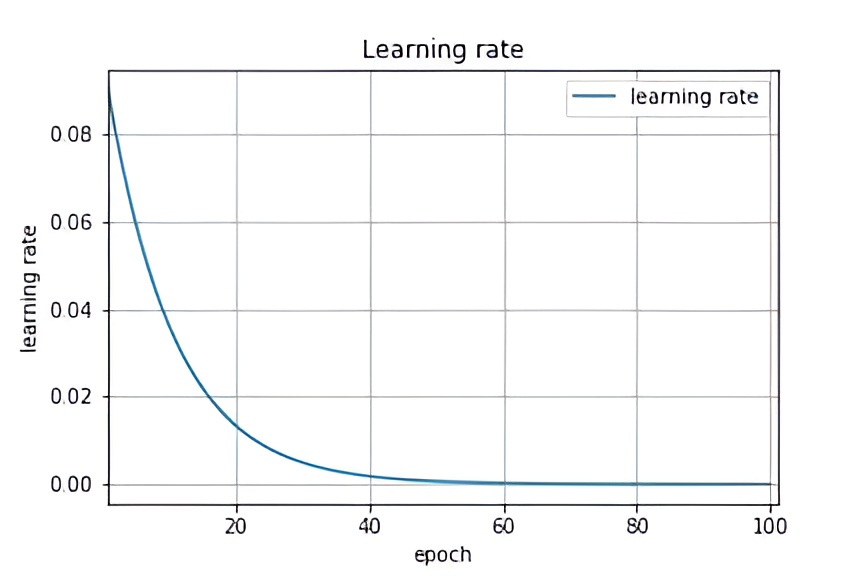
\includegraphics[width=12cm]{gambar/exp.png}
%     \caption{\textit{Exponential Learning Rate Decay.} \textit{Sumber: \citep{suki_lau_2017}}.}
%     \label{exp_lr}
% \end{figure}
%
% Model ini akan dilatih sebanyak 200 epoch dan model dari tiap epoch akan disimpan dalam format file \texttt{h5} agar dapat dipilih model dengan \texttt{val\_loss} (ralat dari set data validasi) terendah dan tidak ada indikasi \textit{overfitting}.
%
% \subsection{Hasil Pelatihan}
% Salah satu cara untuk mendiagnosa \textit{overfitting} dan \textit{underfitting} adalah dengan me-\textit{plot} ralat pelatihan dan ralat validasi \citep{elgendy_2020} atau yang disebut dengan kurva pelatihan (\textit{learning curve}). Kurva pelatihan untuk pelatihan model ini terdapat pada Gambar \ref{learning_curve}
%
% \begin{figure}[h!]
%     \centering
%     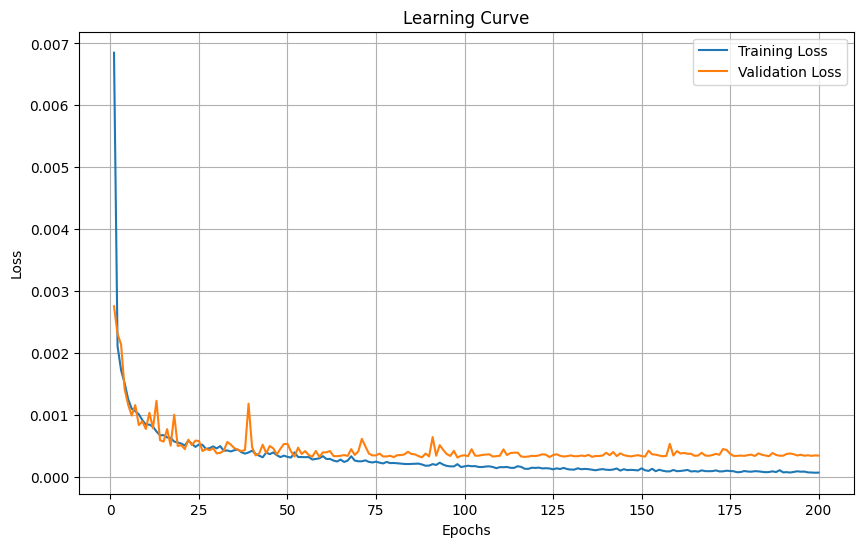
\includegraphics[width=12cm]{gambar/learning_curve.png}
%     \caption{Kurva pemelajaran model. Jumlah ralat pada set data pelatihan dan validasi terhadap jumlah \textit{epoch}}
%     \label{learning_curve}
% \end{figure}
%
% Secara umum, pelatihan ini menghasilkan diagnosa \textit{overfitting} karena model mempelajari set data latih terlalu baik dibandingkan set data validasi \citep{brownlee_2019a}. Hal ini terlihat dari kurva validasi yang berada di atas kurva latih, yang artinya, pada pelatihan terakhir, model menghasilkan ralat validasi yang lebih besar dari pada ralat latih. Walaupun perbedaan ralat di akhir pelatihan relatif kecil, namun munculnya indikasi \textit{overfitting} tidak bisa dinafikan.
%
% Hasil pelatihan ini tetap dapat digunakan dengan cara mencari model terbaik dari \textit{epochs} pelatihan. Salah satu indikasi model tersebut \textit{goodfit} adalah antara kurva validasi dan pelatihan tidak ada jarak (berhimpit) atau kurva validasi berada di bawah kurva latih. Berdasarkan hasil pengamatan, model terbaik adalah model dari \textit{epoch} ke-57 dengan ralat latih : 2.1185e-04 dan ralat validasi: 2.1775e-04.
%
% \section{Hasil Prediksi Jaringan Saraf}
% Prediksi dilakukan menggunakan dua model. Yaitu model dari \textit{epoch} ke-57 dan model dari \textit{epoch} ke-200. Kedua model akan memprediksi dua set data, yaitu set data acak sebanyak 100 data dan set data Gaussian (Persamaan \eqref{gaussian}) sebanyak 18 data.
%
% Setelah melakukan prediksi, hasil prediksi yang sudah dinormalisasi dengan nilai tertinggi dari set data latih (1814160), akan akan diperiksa \textit{mean squared error} (MSE) dan \textit{mean absolute error} (MAE) dari keseluruhan set data dan beberapa medan yang dipilih secara acak dari masing-masing set data uji.
%
% Selain MSE dan MAE, akan diperiksa pula MAPE (Persamaan \eqref{mape}) dari $>1000$ piksel yang nilainya lebih dari 0,1 yang dipilih secara acak. Pemilihan jumlah sampel sebanyak 1000 adalah sesuai dengan rekomendasi dari \cite{israel1992determining} untuk jumlah populasi data 100 $\times$ 100 = 10.000, dibutuhkan setidaknya 1.000 data untuk mendapatkan \textit{margin of error} $\pm 3\%$. Dan untuk pengambilan data di atas 0,1, hal ini karena menurut \cite{DEMYTTENAERE201638}, MAPE lebih cocok untuk mengukur ralat dengan nilai yang jauh dari nol. Salah satu penyebabnya adalah adanya pembagian dengan nilai sebenarnya, yang apabila nilai tersebut nol atau sangat kecil, ralat yang dihasilkan bisa sangat besar, atau intinya, MAPE sangat sensitif terhadap nilai nol atau yang sangat kecil.
%
% \subsection{Hasil Prediksi data Acak 100 Data}
% Dengan menggunakan \textit{solver} Gauss-Seidel C++, waktu yang dibutuhkan untuk menghitung potensial listrik dari 100 data dengan distribusi acak adalah sebesar 325 detik.
%
% \subsubsection{Hasil Prediksi Dengan Model dari \textit{Epoch} ke-200}
% Akan ditinjau terlebih dahulu hasil prediksi menggunakan model dari \textit{epoch} ke-200. Hasil umum dari prediksi 100 data acak dapat dilihat pada Tabel \ref{200acak}.
%
% \begin{table}[h!]
% \centering
% \caption{Hasil keseluruhan prediksi dengan model epoch ke-200 untuk 100 data acak.}
% \label{200acak}
% \begin{tabular}{ll}
% \hline
% \textbf{Metrik}        & \textbf{Nilai}         \\ \hline
% Waktu prediksi (detik) & 3                      \\ \hline
% MSE                    & 0.00023130870479720733 \\ \hline
% MAE                    & 0.0105920327822764     \\ \hline
% \end{tabular}
% \end{table}
%
% Kemudian disajikan hasil visual dari 3 medan yang dipilih secara acak beserta dengan rerata ralatnya
% \begin{enumerate}
%     \item Data ke-0
%     
%     mean absolute error medan =  0.011185391142800172\\
%     mean squared error medan = 0.0002198482412056808\\
%     mape sampling =  6.652328247576015
%     \begin{figure}[h!]
%     \centering
%     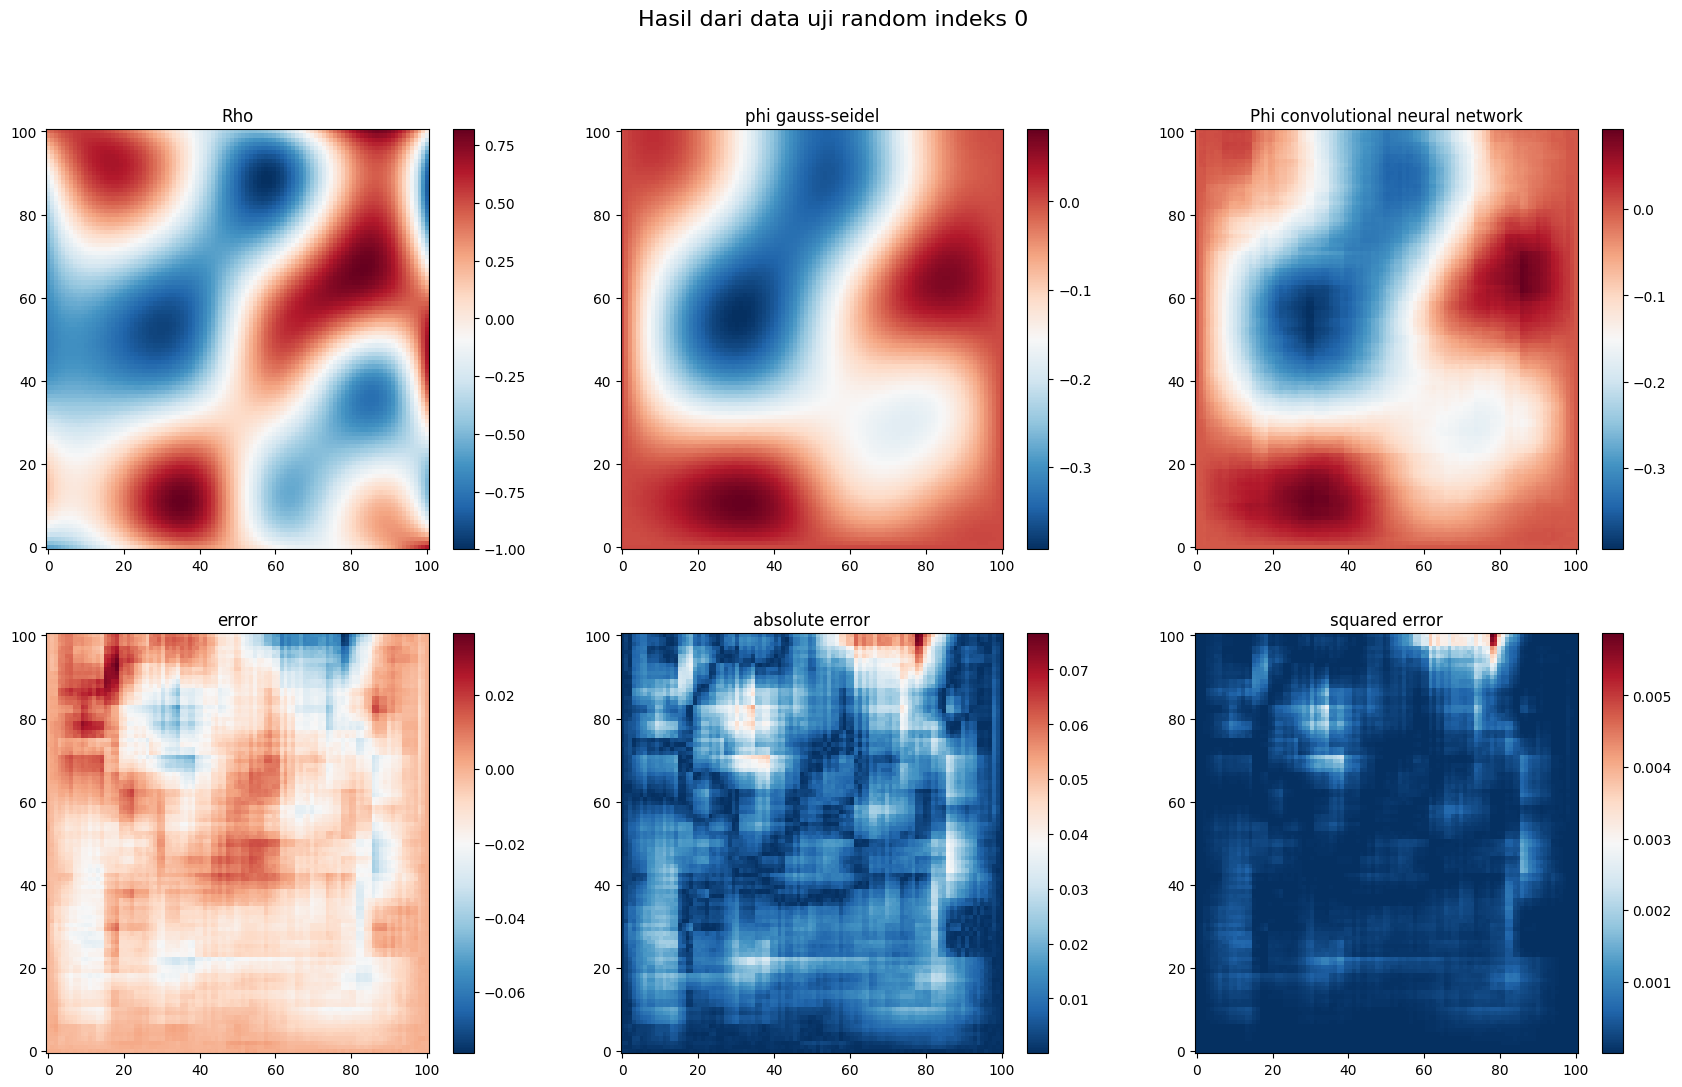
\includegraphics[width=12cm]{gambar/0_200_acak.png}
%     \caption{Hasil visual prediksi dengan model dari epoch ke-200 untuk set data acak, indeks ke-0}
%     \label{0_200_acak}
%     \end{figure}
%
%     \item Data ke-40
%
%     mean absolute error medan =  0.013264649605893237\\
%     mean squared error medan =  0.00027769889839297595\\
%     mape sampling =  -7.139269391922416
%     \begin{figure}[h!]
%     \centering
%     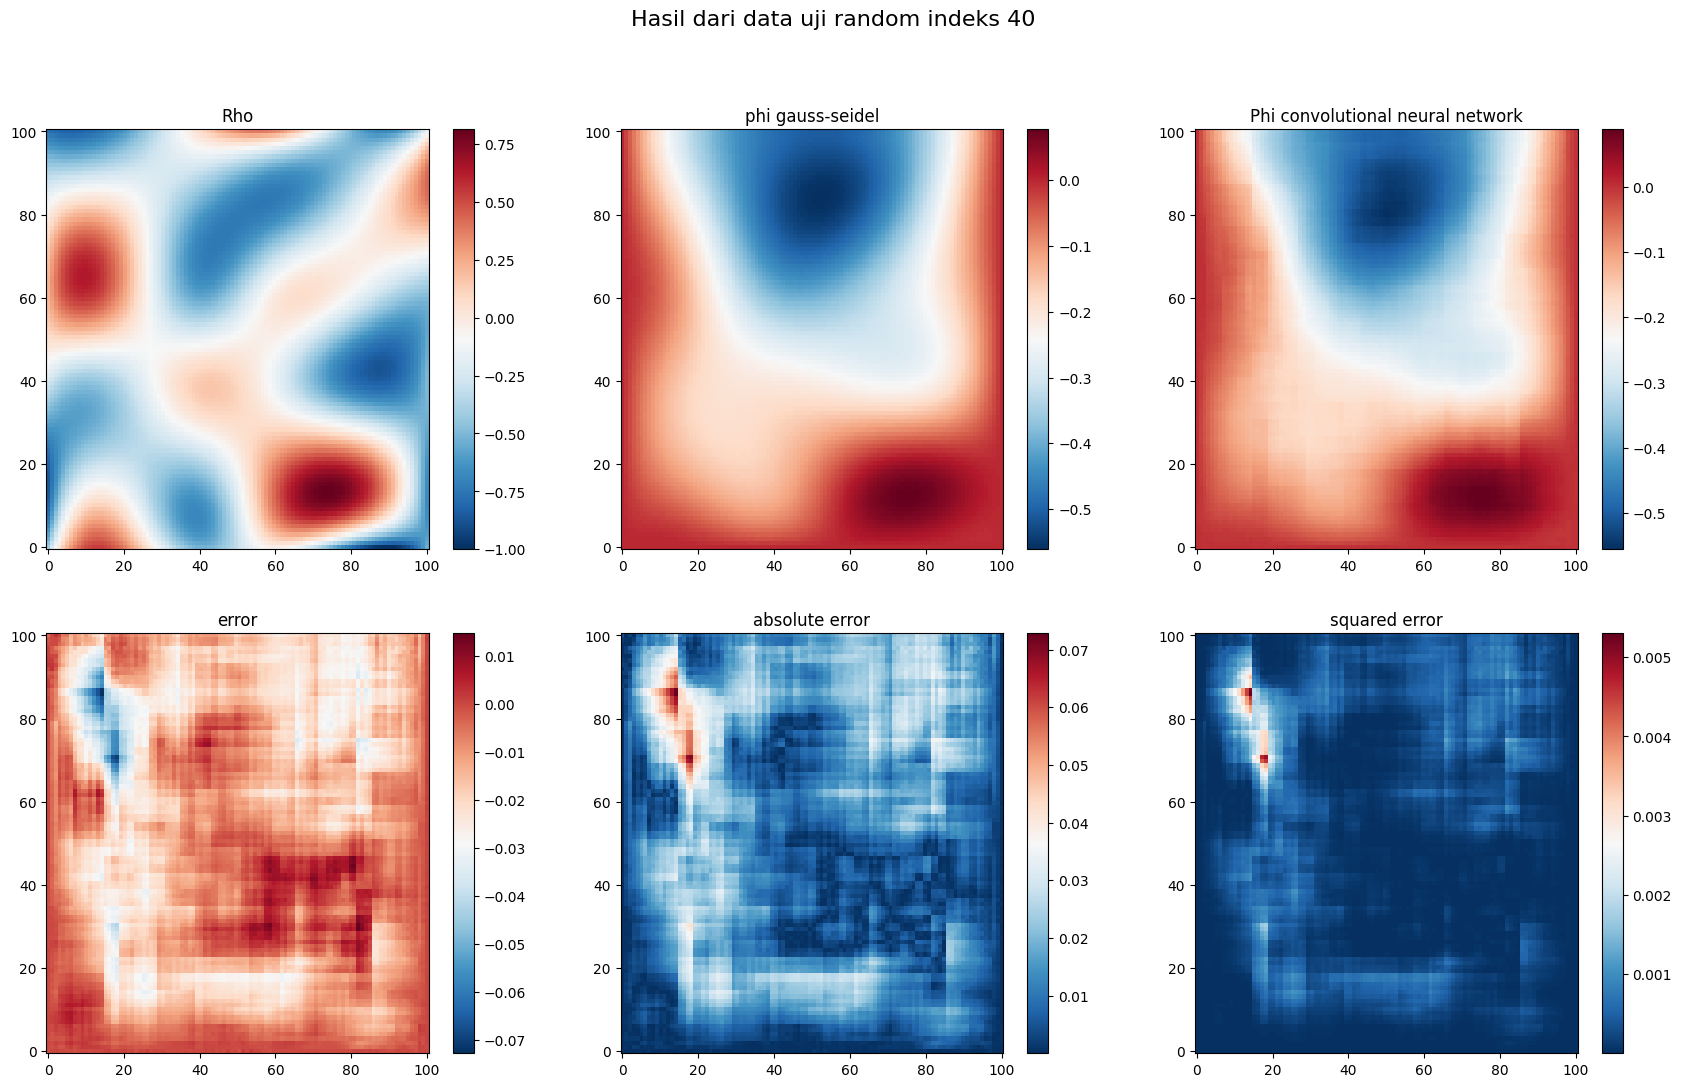
\includegraphics[width=12cm]{gambar/40_200_acak.png}
%     \caption{Hasil visual prediksi dengan model dari epoch ke-200 untuk set data acak, indeks ke-40}
%     \label{40_200_acak}
%     \end{figure}
%
%     \item Data ke-42
%     mean absolute error medan =  0.009555791057188687\\
%     mean squared error medan = 0.0001709383632965548\\
%     mape sampling =  15.947304897803454
%     \begin{figure}[h!]
%     \centering
%     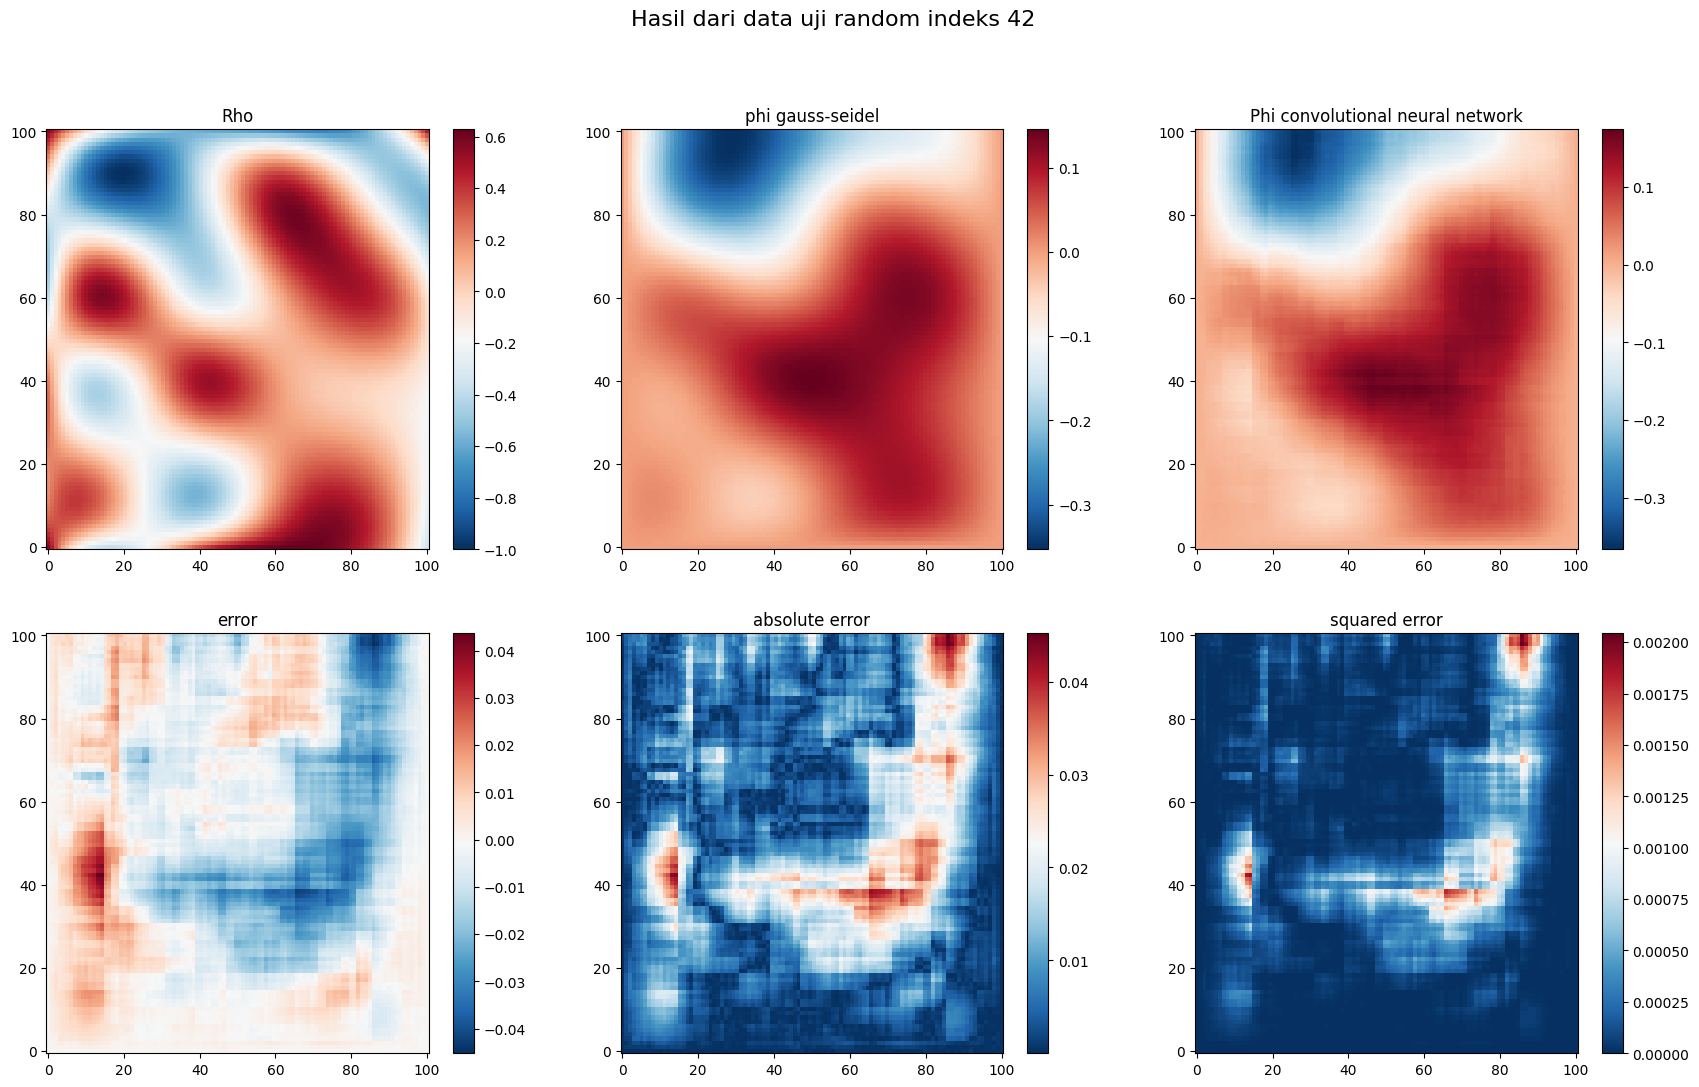
\includegraphics[width=12cm]{gambar/42_200_acak.png}
%     \caption{Hasil visual prediksi dengan model dari epoch ke-200 untuk set data acak, indeks ke-42}
%     \label{42_200_acak}
%     \end{figure}
%     
% \end{enumerate}
%
% \subsubsection{Hasil Prediksi Dengan Model dari \textit{Epoch} ke-57}
% Akan ditinjau terlebih dahulu hasil prediksi menggunakan model dari \textit{epoch} ke-57. Hasil umum dari prediksi 100 data acak dapat dilihat pada Tabel \ref{57acak}.
%
% \begin{table}[h!]
% \centering
% \caption{Hasil keseluruhan prediksi dengan model epoch ke-57 untuk 100 data acak.}
% \label{57acak}
% \begin{tabular}{ll}
% \hline
% \textbf{Metrik}        & \textbf{Nilai}         \\ \hline
% Waktu prediksi (detik) & 2                      \\ \hline
% MSE                    & 0.0002451981196005638 \\ \hline
% MAE                    & 0.011251571534445289     \\ \hline
% \end{tabular}
% \end{table}
%
% Kemudian disajikan hasil visual dari 3 medan yang dipilih secara acak beserta dengan rerata ralatnya
% \begin{enumerate}
%     \item Data ke-0
%     
%     mean absolute error medan =  0.013908464504802816\\
%     mean squared error medan =  0.000344087854795096\\
%     mape sampling =  -8.33244489614455
%     \begin{figure}[h!]
%     \centering
%     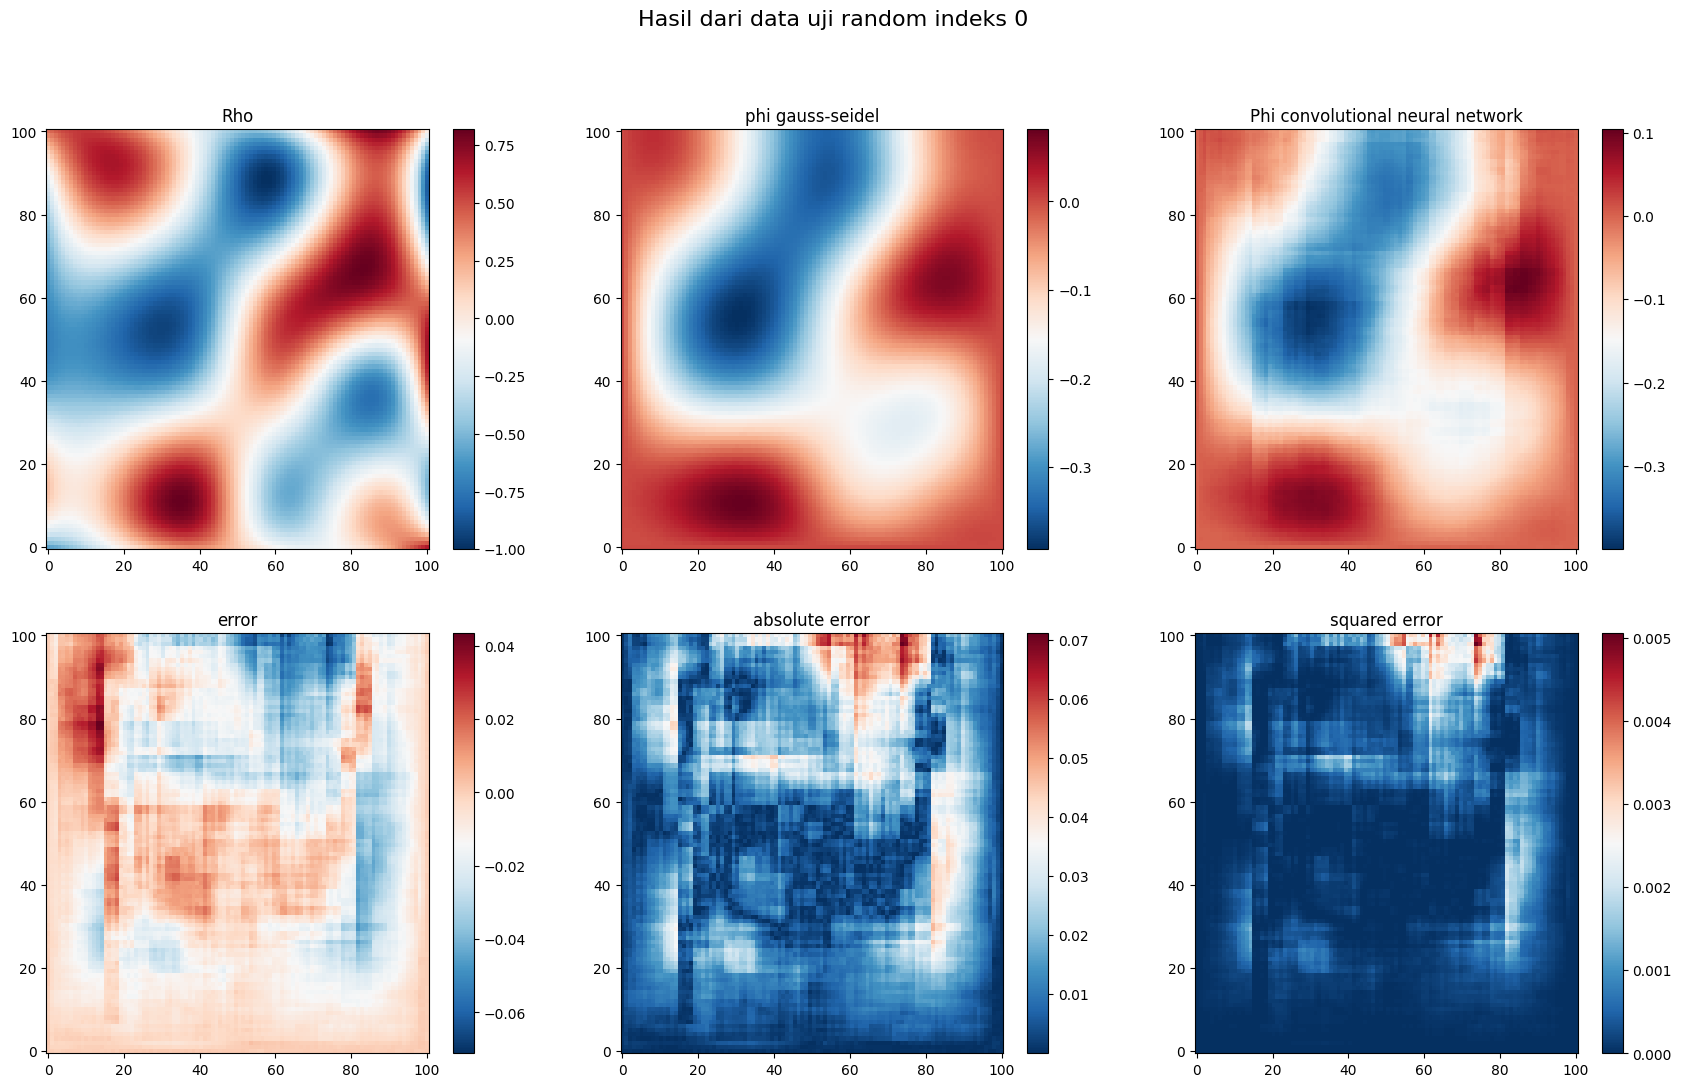
\includegraphics[width=12cm]{gambar/0_57_acak.png}
%     \caption{Hasil visual prediksi dengan model dari epoch ke-57 untuk set data acak, indeks ke-0}
%     \label{0_57_acak}
%     \end{figure}
%
%     \item Data ke-40
%
%     mean absolute error medan =  0.014362610343673214\\
%     mean squared error medan =  0.00030545219599322355\\
%     mape sampling =  -7.8525725979344605
%     \begin{figure}[h!]
%     \centering
%     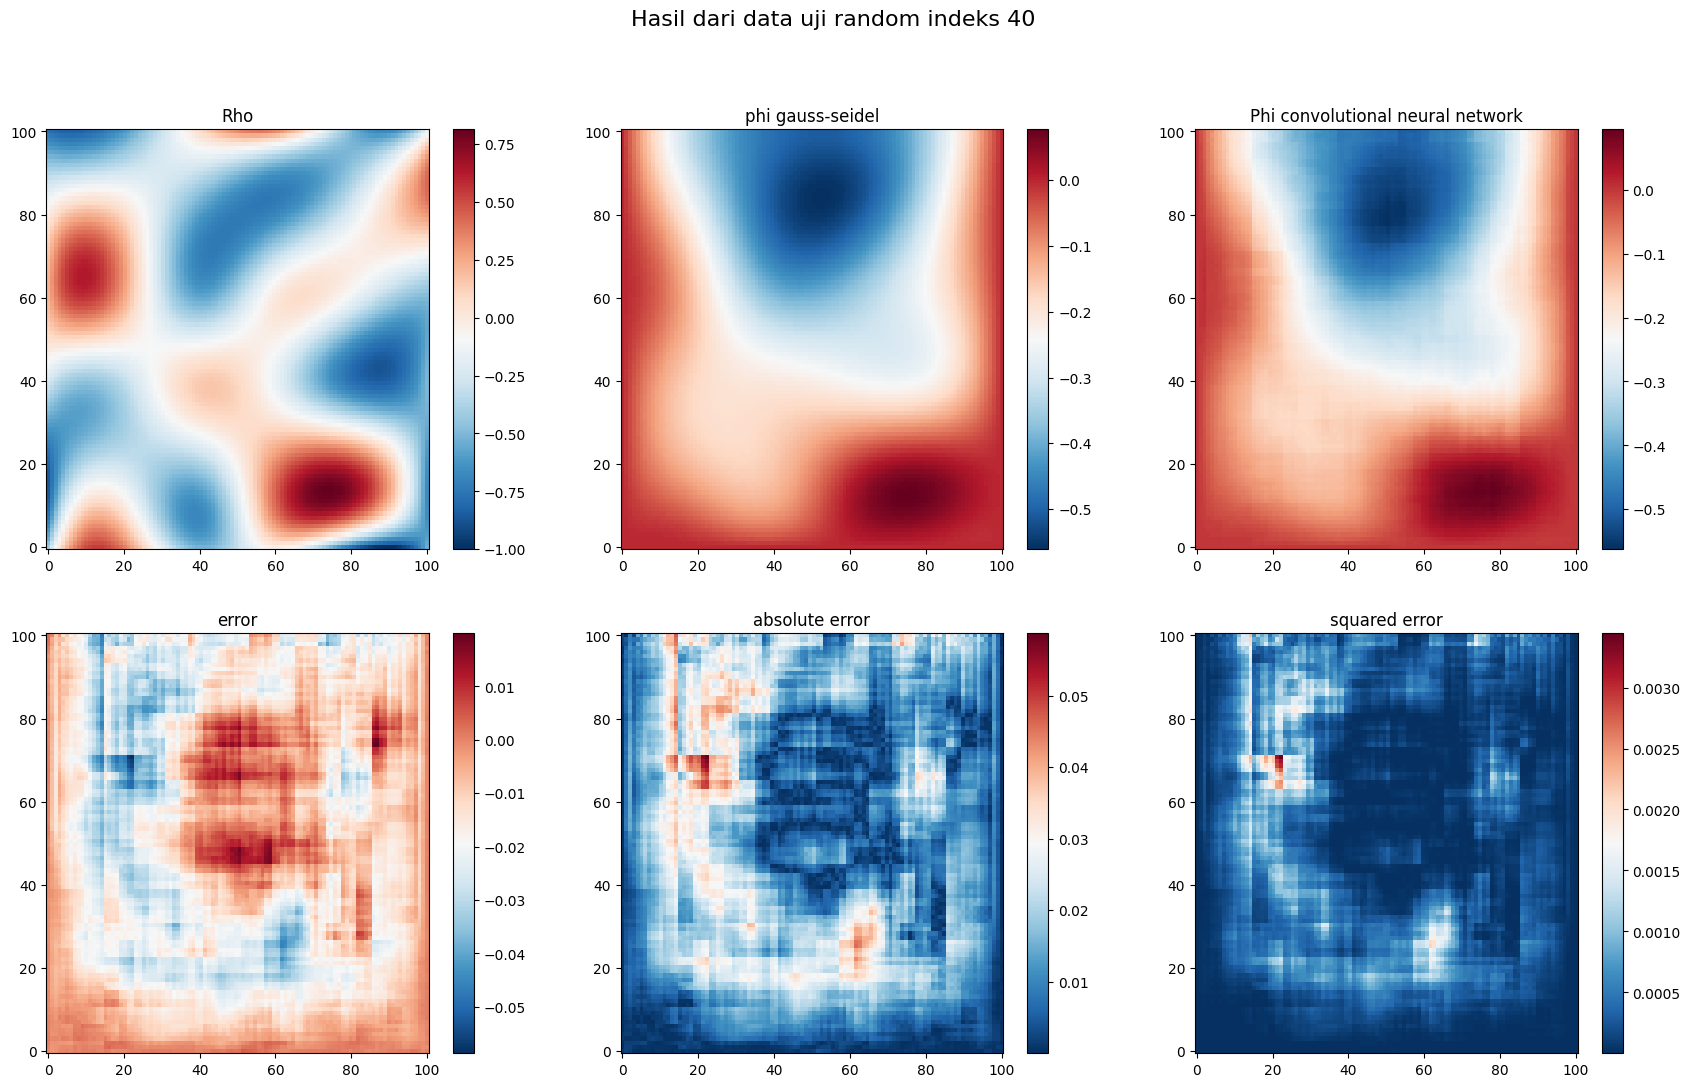
\includegraphics[width=12cm]{gambar/40_57_acak.png}
%     \caption{Hasil visual prediksi dengan model dari epoch ke-57 untuk set data acak, indeks ke-40}
%     \label{40_57_acak}
%     \end{figure}
%
%     \item Data ke-42
%     mean absolute error medan =  0.01258524854440124\\
%     mean squared error medan =  0.0002786093680182126\\
%     mape sampling =  21.275292145676676
%     \begin{figure}[h!]
%     \centering
%     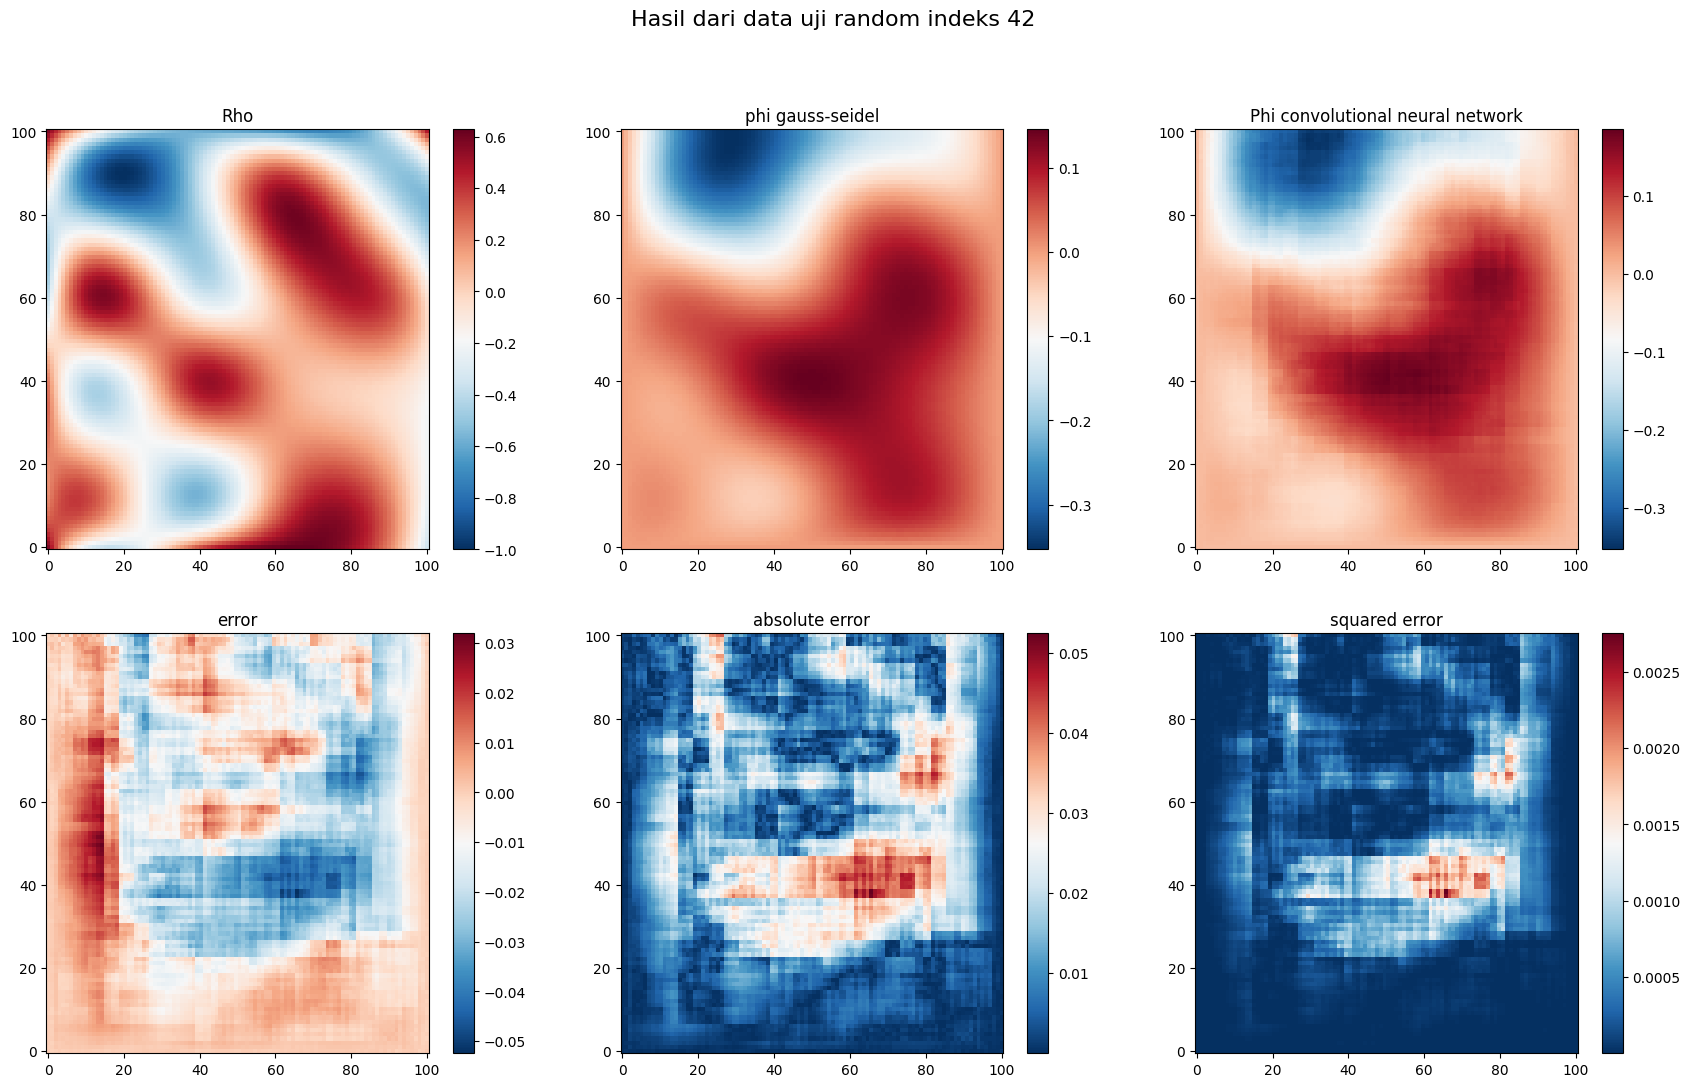
\includegraphics[width=12cm]{gambar/42_57_acak.png}
%     \caption{Hasil visual prediksi dengan model dari epoch ke-57 untuk set data acak, indeks ke-42}
%     \label{42_57_acak}
%     \end{figure}
%     
% \end{enumerate}
%
% \subsection{Hasil Prediksi data Gaussian 18 Data}
% Dengan menggunakan \textit{solver} Gauss-Seidel C++, waktu yang dibutuhkan untuk menghitung potensial listrik dari 18 data dengan distribusi Gaussian adalah sebesar 45 detik.
%
% \subsubsection{Hasil Prediksi Dengan Model dari \textit{Epoch} ke-200}
% Akan ditinjau terlebih dahulu hasil prediksi menggunakan model dari \textit{epoch} ke-200. Hasil umum dari prediksi 18 data Gaussian dapat dilihat pada Tabel \ref{200acak}.
%
% \begin{table}[h!]
% \centering
% \caption{Hasil keseluruhan prediksi dengan model epoch ke-200 untuk 18 data Gaussian.}
% \label{200gaussian}
% \begin{tabular}{ll}
% \hline
% \textbf{Metrik}        & \textbf{Nilai}         \\ \hline
% Waktu prediksi (detik) & 0                      \\ \hline
% MSE                    & 0.0004893961671139401 \\ \hline
% MAE                    & 0.014389271830866605  \\ \hline
% \end{tabular}
% \end{table}
%
% Kemudian disajikan hasil visual dari 3 medan yang dipilih secara acak beserta dengan rerata ralatnya
% \begin{enumerate}
%     \item Data ke-6
%     mean absolute error medan = 0.009043942980161843\\
%     mean squared error medan = 0.00017162983257671422\\
%     mape sampling = 4.7754985462483495
%     \begin{figure}[h!]
%     \centering
%     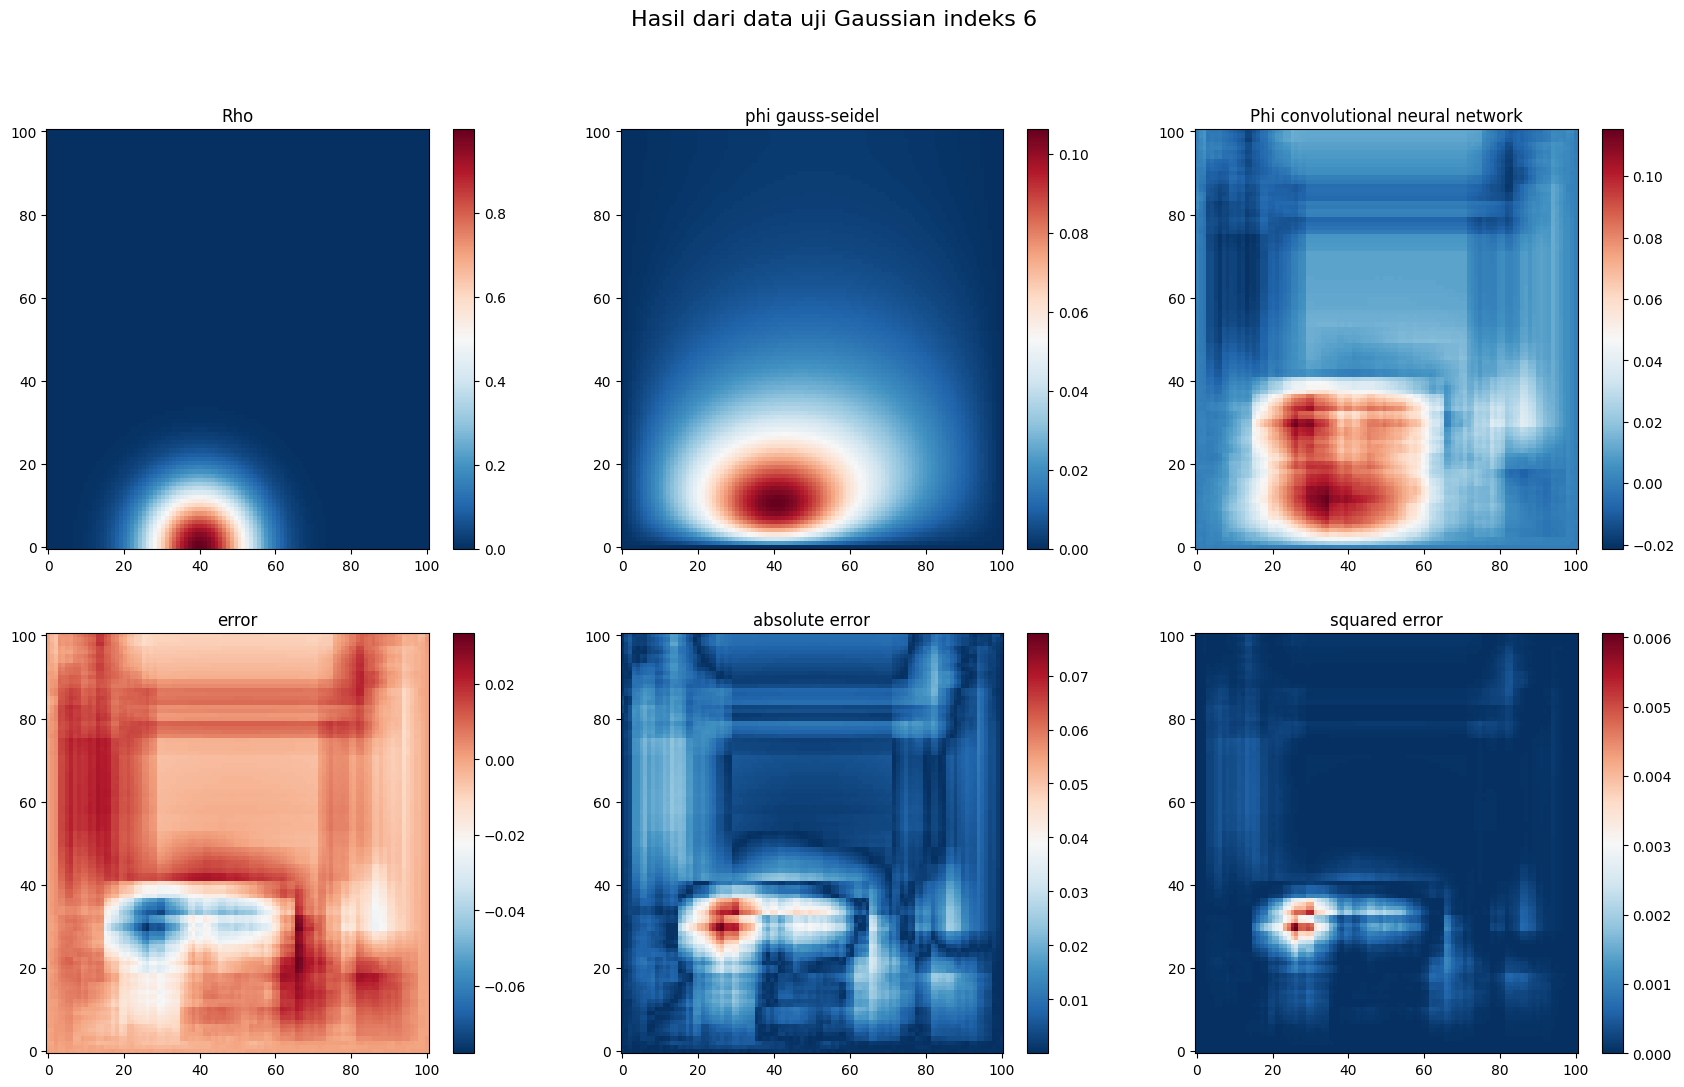
\includegraphics[width=12cm]{gambar/6_200_gaussian.png}
%     \caption{Hasil visual prediksi dengan model dari epoch ke-200 untuk set data Gaussian, indeks ke-6}
%     \label{6_200_Gaussian}
%     \end{figure}
%
%     \item Data ke-10
%     mean absolute error medan = 0.021639103274408242\\
%     mean squared error medan = 0.0007739544987668907\\
%     mape sampling = 15.772617188907128
%     \begin{figure}[h!]
%     \centering
%     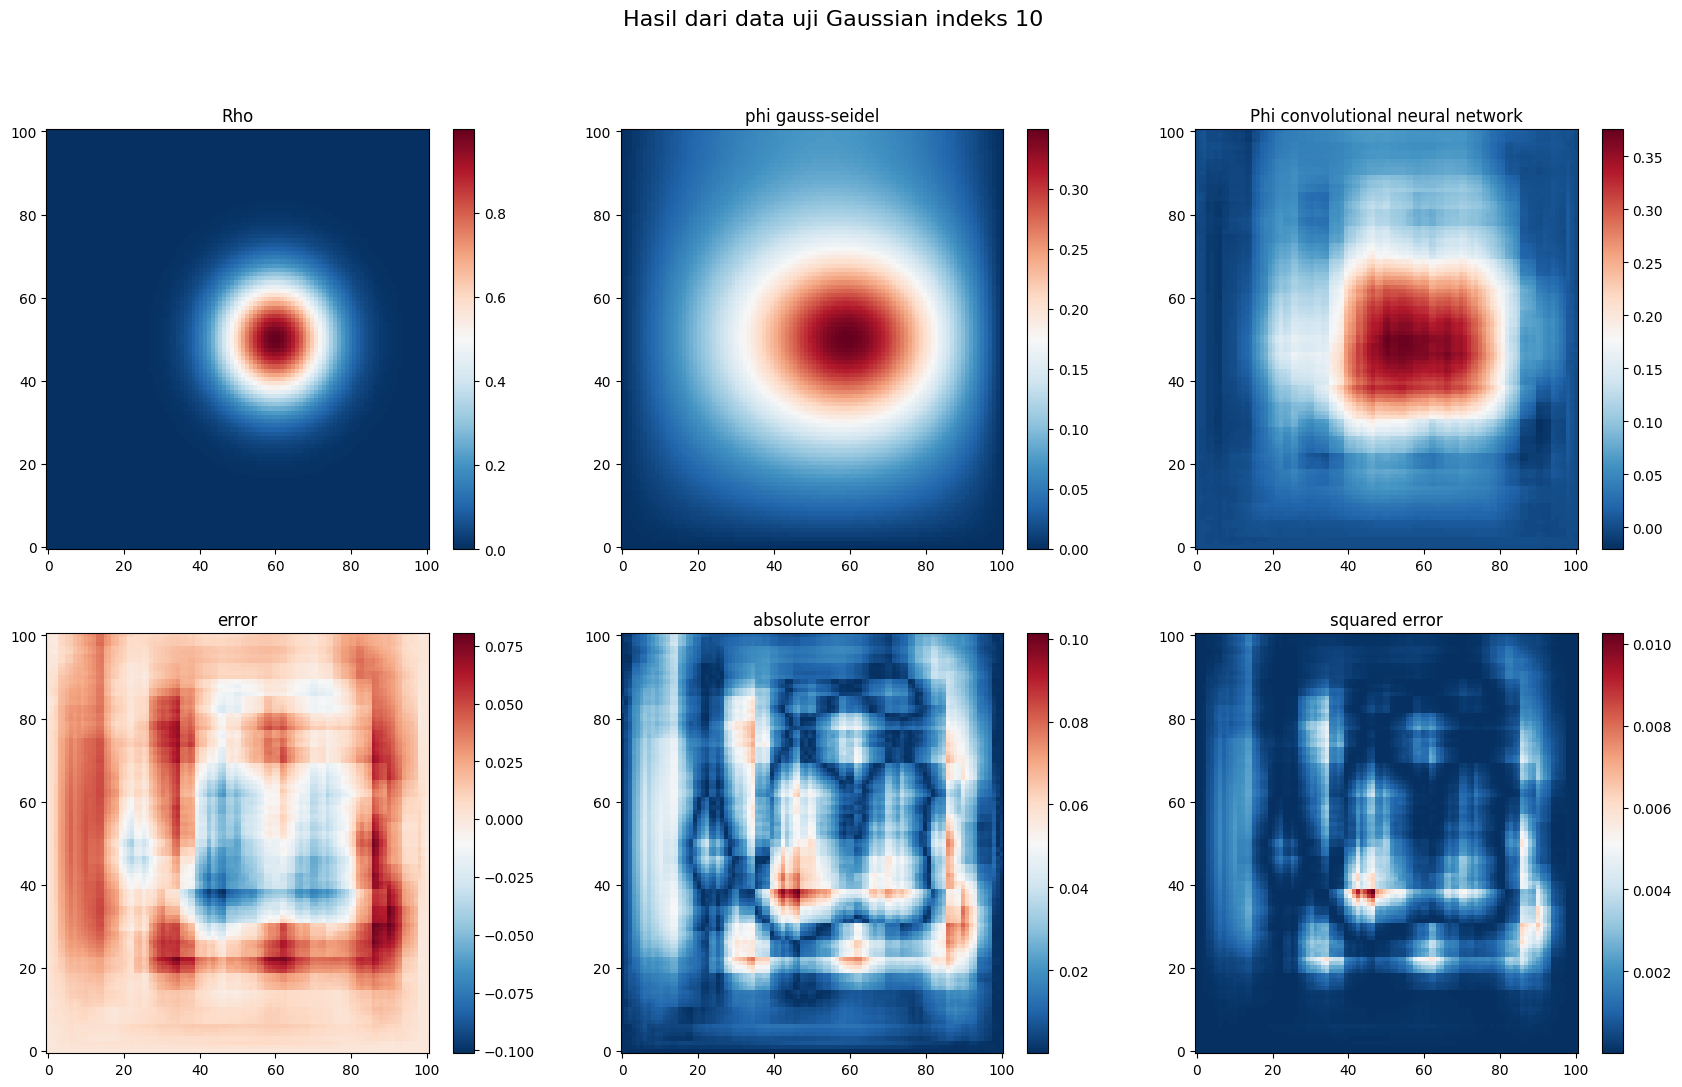
\includegraphics[width=12cm]{gambar/10_200_gaussian.png}
%     \caption{Hasil visual prediksi dengan model dari epoch ke-200 untuk set data Gaussian, indeks ke-10}
%     \label{10_200_Gaussian}
%     \end{figure}
%
%     \item Data ke-4
%     mean absolute error medan =  0.025968039199870924\\
%     mean squared error medan = 0.0011480142622138615\\
%     mape sampling =  29.026637482792307
%     \begin{figure}[h!]
%     \centering
%     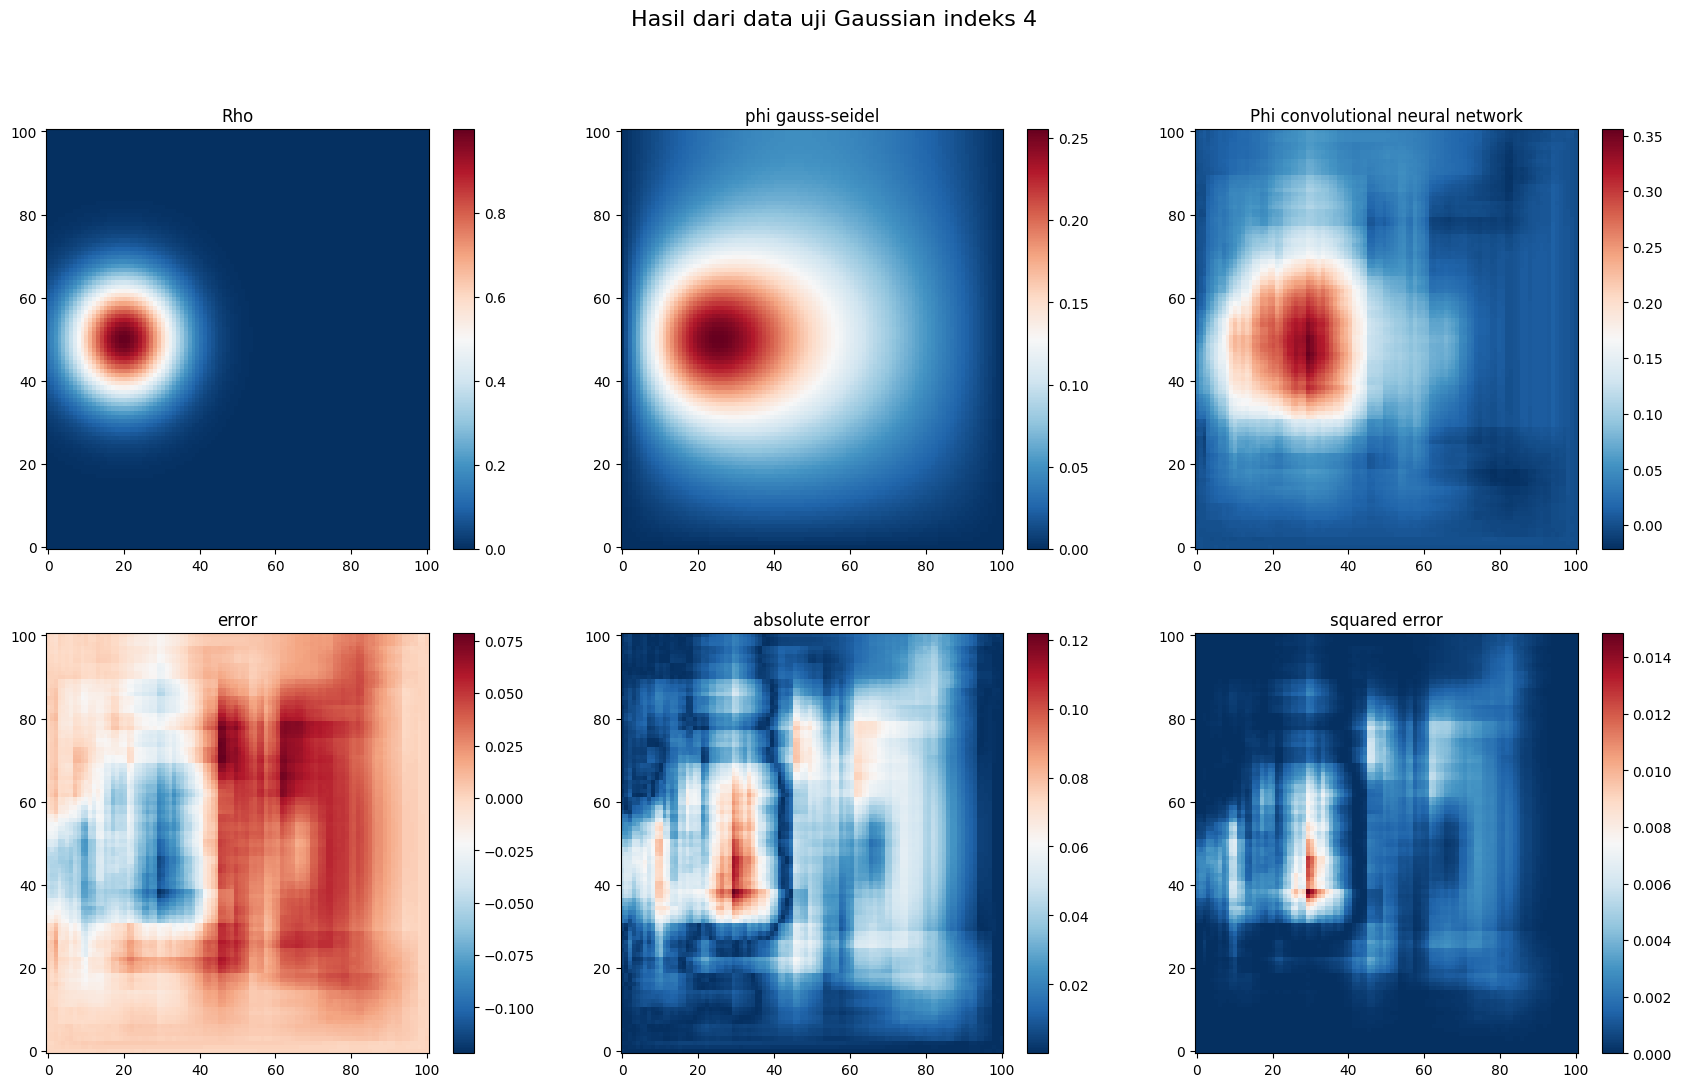
\includegraphics[width=12cm]{gambar/4_200_gaussian.png}
%     \caption{Hasil visual prediksi dengan model dari epoch ke-200 untuk set data Gaussian, indeks ke-4}
%     \label{4_200_gaussian}
%     \end{figure}
%     
% \end{enumerate}
%
% \subsubsection{Hasil Prediksi Dengan Model dari \textit{Epoch} ke-57}
% Akan ditinjau terlebih dahulu hasil prediksi menggunakan model dari \textit{epoch} ke-57. Hasil umum dari prediksi 18 data Gaussian dapat dilihat pada Tabel \ref{57gaussian}.
%
% \begin{table}[h!]
% \centering
% \caption{Hasil keseluruhan prediksi dengan model epoch ke-57 untuk 18 data Gaussian.}
% \label{57gaussian}
% \begin{tabular}{ll}
% \hline
% \textbf{Metrik}        & \textbf{Nilai}         \\ \hline
% Waktu prediksi (detik) & 0                      \\ \hline
% MSE                    & 0.0004993306540695422 \\ \hline
% MAE                    & 0.014593957448582126     \\ \hline
% \end{tabular}
% \end{table}
%
% Kemudian disajikan hasil visual dari 3 medan yang dipilih secara acak beserta dengan rerata ralatnya
% \begin{enumerate}
%     \item Data ke-6
%     
%     mean absolute error medan =  0.011164339060049471\\
%     mean squared error medan =  0.0003275269746363096\\
%     mape sampling =  4.860758654485836
%     \begin{figure}[h!]
%     \centering
%     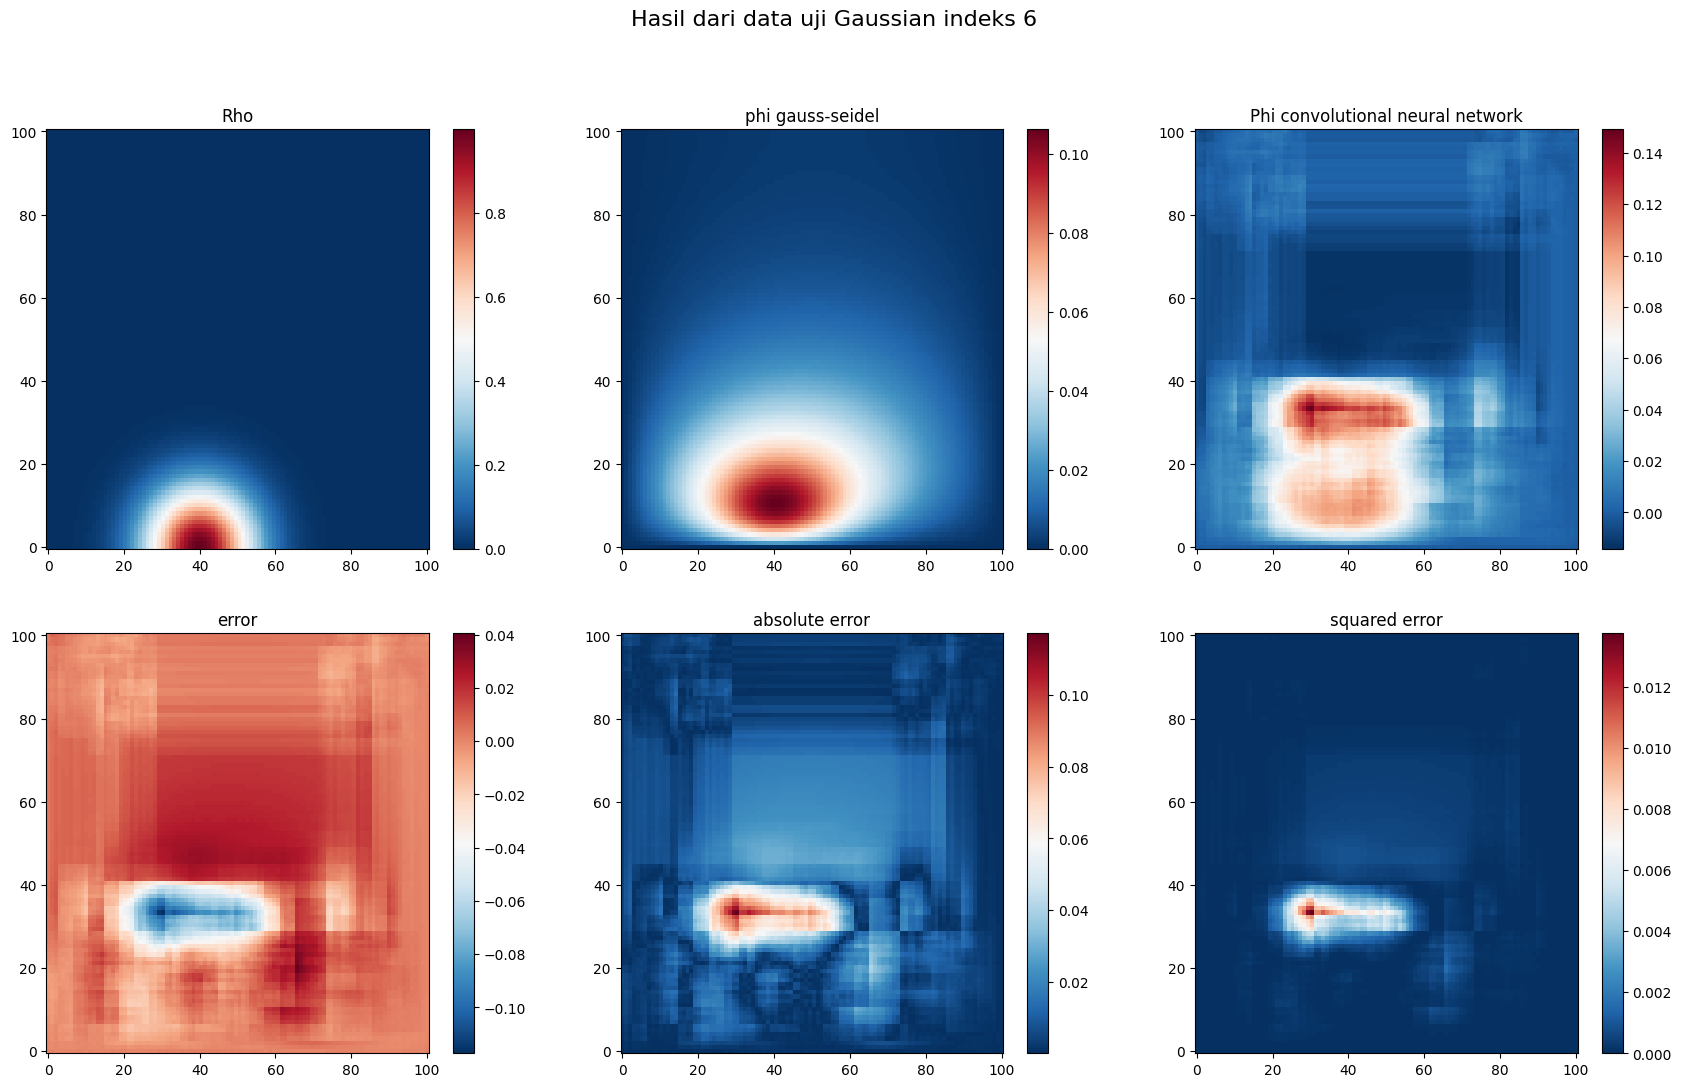
\includegraphics[width=12cm]{gambar/6_57_gaussian.png}
%     \caption{Hasil visual prediksi dengan model dari epoch ke-57 untuk set data Gaussian, indeks ke-6}
%     \label{0_57_acak}
%     \end{figure}
%
%     \item Data ke-10
%     mean absolute error medan = 0.020210462134109868\\
%     mean squared error medan = 0.0006902836080606566\\
%     mape sampling =  17.241594270499036
%     \begin{figure}[h!]
%     \centering
%     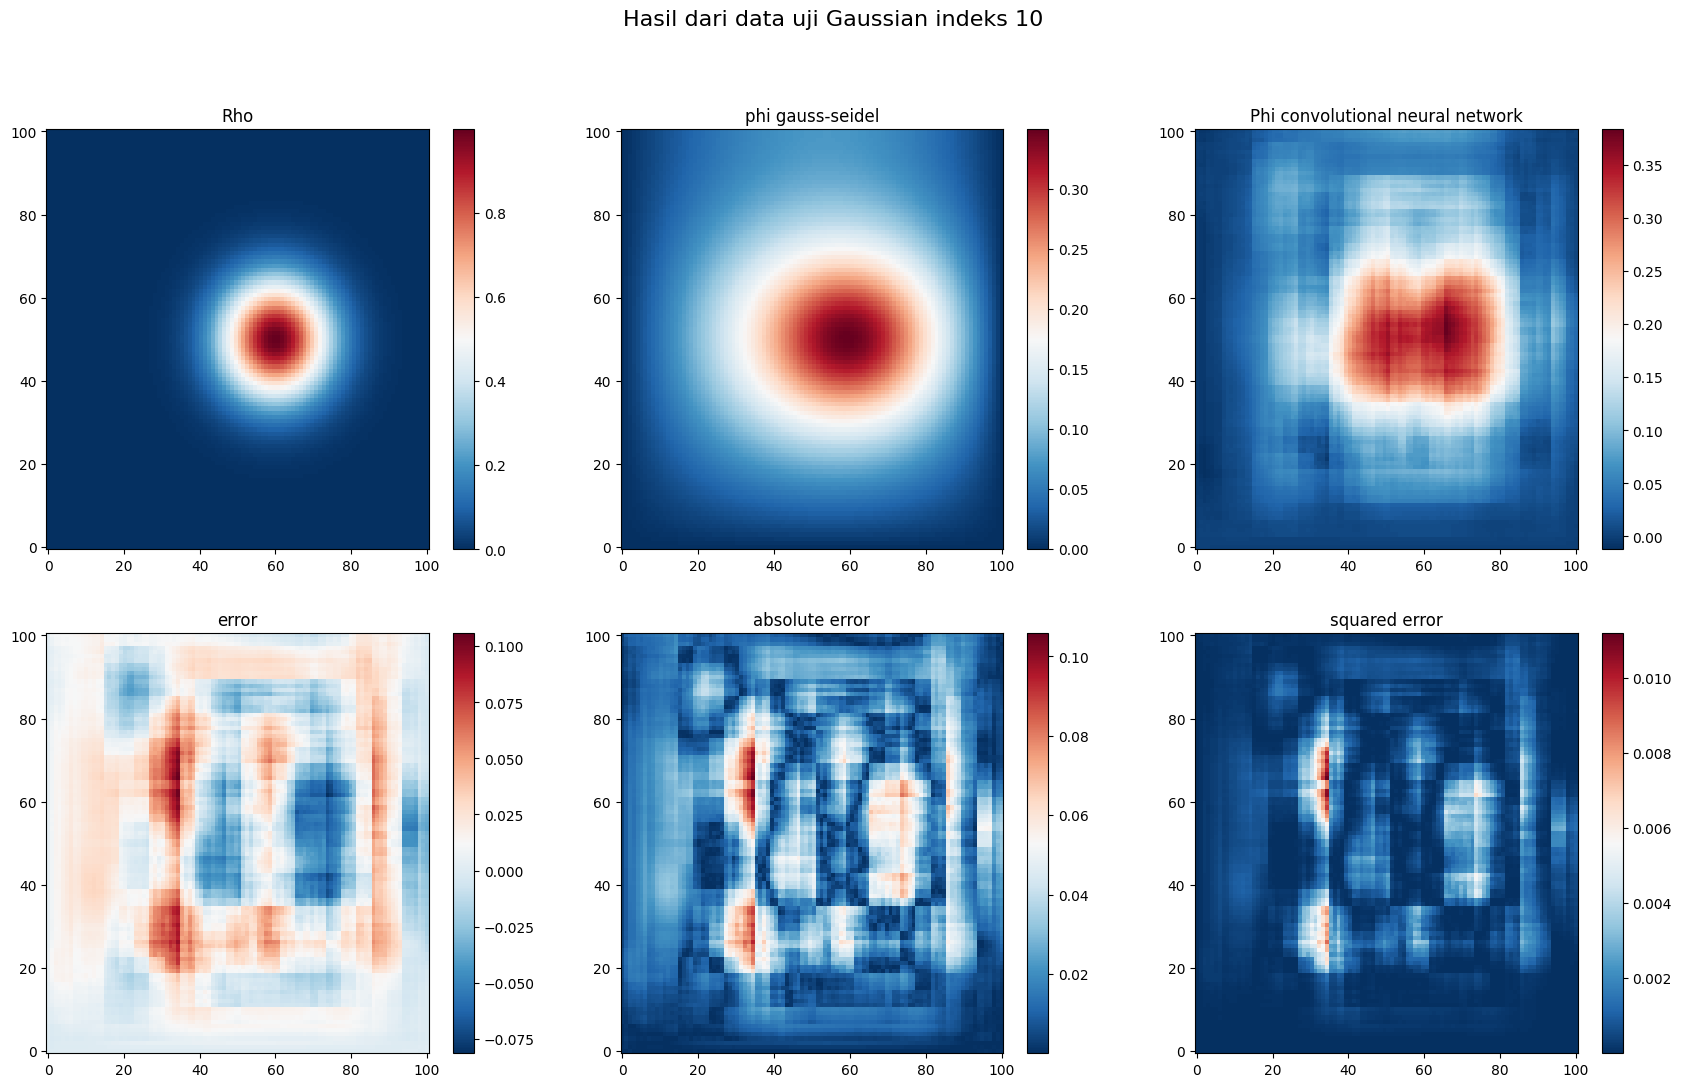
\includegraphics[width=12cm]{gambar/10_57_gaussian.png}
%     \caption{Hasil visual prediksi dengan model dari epoch ke-57 untuk set data Gaussian, indeks ke-10}
%     \label{10_57_acak}
%     \end{figure}
%
%     \item Data ke-4
%     mean absolute error medan =  0.02386963821168969\\
%     mean squared error medan =  0.0010337360801227914\\
%     mape sampling =  25.63144233512775
%     \begin{figure}[h!]
%     \centering
%     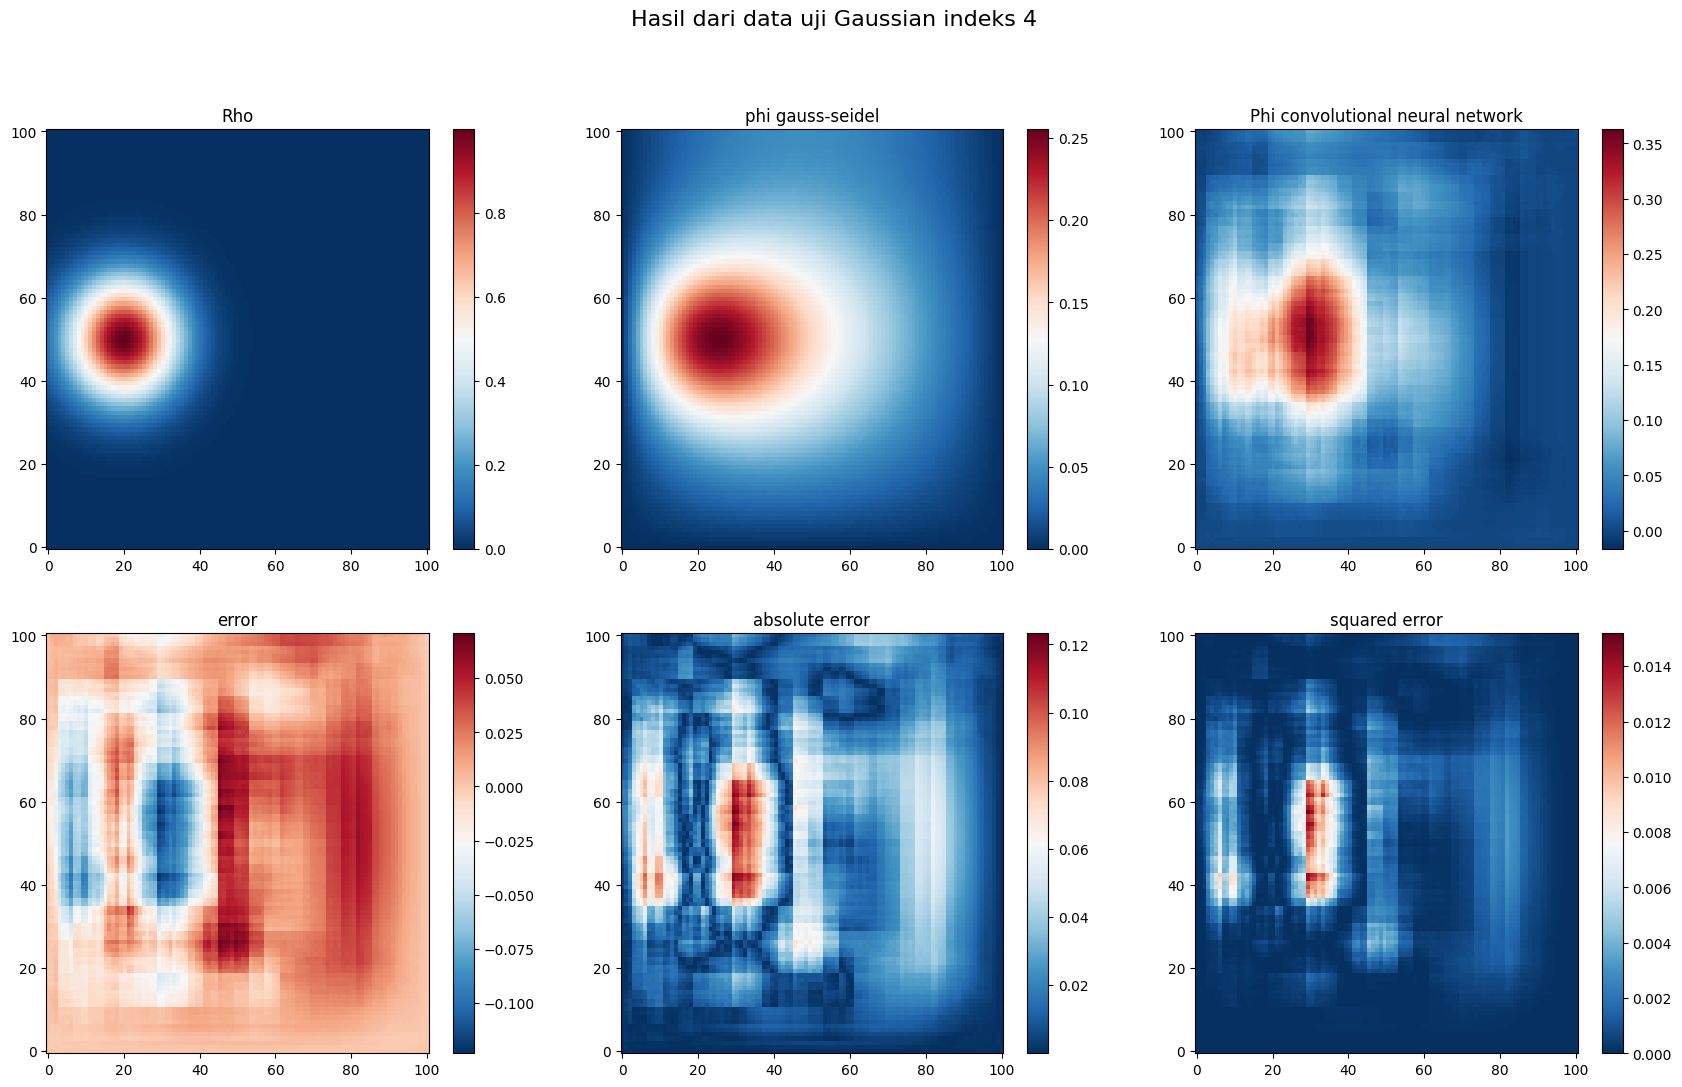
\includegraphics[width=12cm]{gambar/4_57_gaussian.png}
%     \caption{Hasil visual prediksi dengan model dari epoch ke-57 untuk set data Gaussian, indeks ke-4}
%     \label{4_57_Gaussian}
%     \end{figure}
%     
% \end{enumerate}
%
% \section{Pembahasan Secara Umum}
%
% Dari pengamatan visual, dapat diklaim bahwa model yang telah dilatih dapat memberikan gambaran umum yang sesuai dengan visual \textit{ground truth} yang didapat dari metode Gauss-Seidel, terutama pada set data dari data acak. Hal ini sangat masuk akal, mengingat model ini dilatih menggunakan set data latih acak. Untuk kemampuan model memprediksi data distribusi lain, perlu adanya penambahan jenis distribusi lain ke set data latih atau membangun model lain dengan set data latih yang spesifik.
%
% Untuk waktu perhitungan, misalnya waktu perhitungan yang paling tinggi, menggunakan model dari \textit{epoch} ke-200 untuk 100 data distribusi acak memakan waktu 3 detik yang berarti sama dengan perhitungan untuk 1 medan menggunakan \textit{solver} Gauss-Seidel yang digunakan untuk membuat set data latih. Secara keseluruhan, model ini 162,5 $\times$ lebih cepat dalam hal waktu perhitungan.
%
% Dari segi ralat, rerata ralat mutlak dan rerata ralat absolut sudah relatif kecil. Dari visual ralatpun sudah terlihat mayoritas berkonsentrasi rendah, dan hanya meninggi pada distribusi di syarat batas Neumann, misalnya Gambar \ref{0_57_acak}. Untuk MAPE, meski dapat diperdebatkan relativitas besar kecilnya, penulis memiliki pandangan bahwa model dapat menghasilkan MAPE yang relatif kecil. Hal ini karena, pertama, MAPE memang ralat yag tepat digunakan untuk model regresi. Namun, MAPE memang memiliki beberapa kelemahan, beberapa diantaranya adalah MAPE bergantung pada situasi, derajat variabilitas data, rentang nilai sebenarnya, serta \textit{outliers}. Data uji dan data latih yang digunakan masih memiliki beberapa kelemahan, salah satunya adalah bilangan pernormalisir yang jumlahnya tidak mewakili jumlah data yang memiliki nilai tertinggi di sekitar nilai penormalisir. Sehingga sangat memungkinkan ada pergeseran distribusi. Akan lebih memungkinkan apabila ada upaya \textit{data cleaning} seperti misalnya membuang beberapa \textit{tail} data yang nilai ekstrimnya berada jauh dari pusat distribusi sehingga bilangan penormalisirnya bisa lebih mewakili keseluruhan data. Hal tersebut tidak dilakukan karena penulis melihat pada upaya pertama, hasil yang diperoleh sudah cukup bagus dari metrik ralat yang lain dan dari pengamatan visual.
%
% Masih mengenai kelemahan MAPE, MAPE memiliki bias pada hasil prediksi yang berada di bawah nilai \textit{ground truth} \citep{roberts_2023b}. Namun meski begitu, MAPE memberikan gambaran proporsi mengenai ralat dari prediksi terhadap nilai sebenarnya. Sehingga masih relevan untuk digunakan untuk mengukur kemampuan model yang dibangun. Hanya saja memang harus ada upaya untuk memilih data yang akan dijadikan komponen pengukuran, seperti upaya sampling $>1000$ data pada medan yang diukur. 
%
% Beberapa medan hasil yang tidak ditampilkan di sini, ada beberapa medan yang memiliki nilai MAPE dari hasil sampling sebesar kira-kira 3--5\%. Memang hal ini tidak dapat sepenuhnya mengatakan bahwa model ini dapat digunakan sebagai pengganti metode numerik yang sudah mapan, namun dapat mengatakan bahwa model yang dibangun dan dilatih ini dapat mendekati hasil aslinya. Sebagai perbandingan, \cite{Ozbay2021} dapat membangun model untuk 2D dan 3D pada koordinat kartesian yang menghasilkan MAPE di bawah 3\%.
%
% Pada penelitian ini, disajikan 2 model. Berdasarkan pengamatan MSE dari 10 medan yang dihitung menggunakan masing-masing model (Gambar \ref{mse2model}, menunjukkan bahwa kedua model dapat menghasilkan dapat unggul dengan jumlah yang berimbang, artinya, model 57 unggul di 5 kali percobaan, dan model 200 unggul di 5 percobaan juga. Hal ini dapat menggiring pada kesimpulan bahwa meski model 200 memiliki indikasi \textit{overfitting}, namun karena ralat latihnya relatif lebih kecil, model 200 tetap dapat diandalkan. 
% \begin{figure}[h!]
%     \centering
%     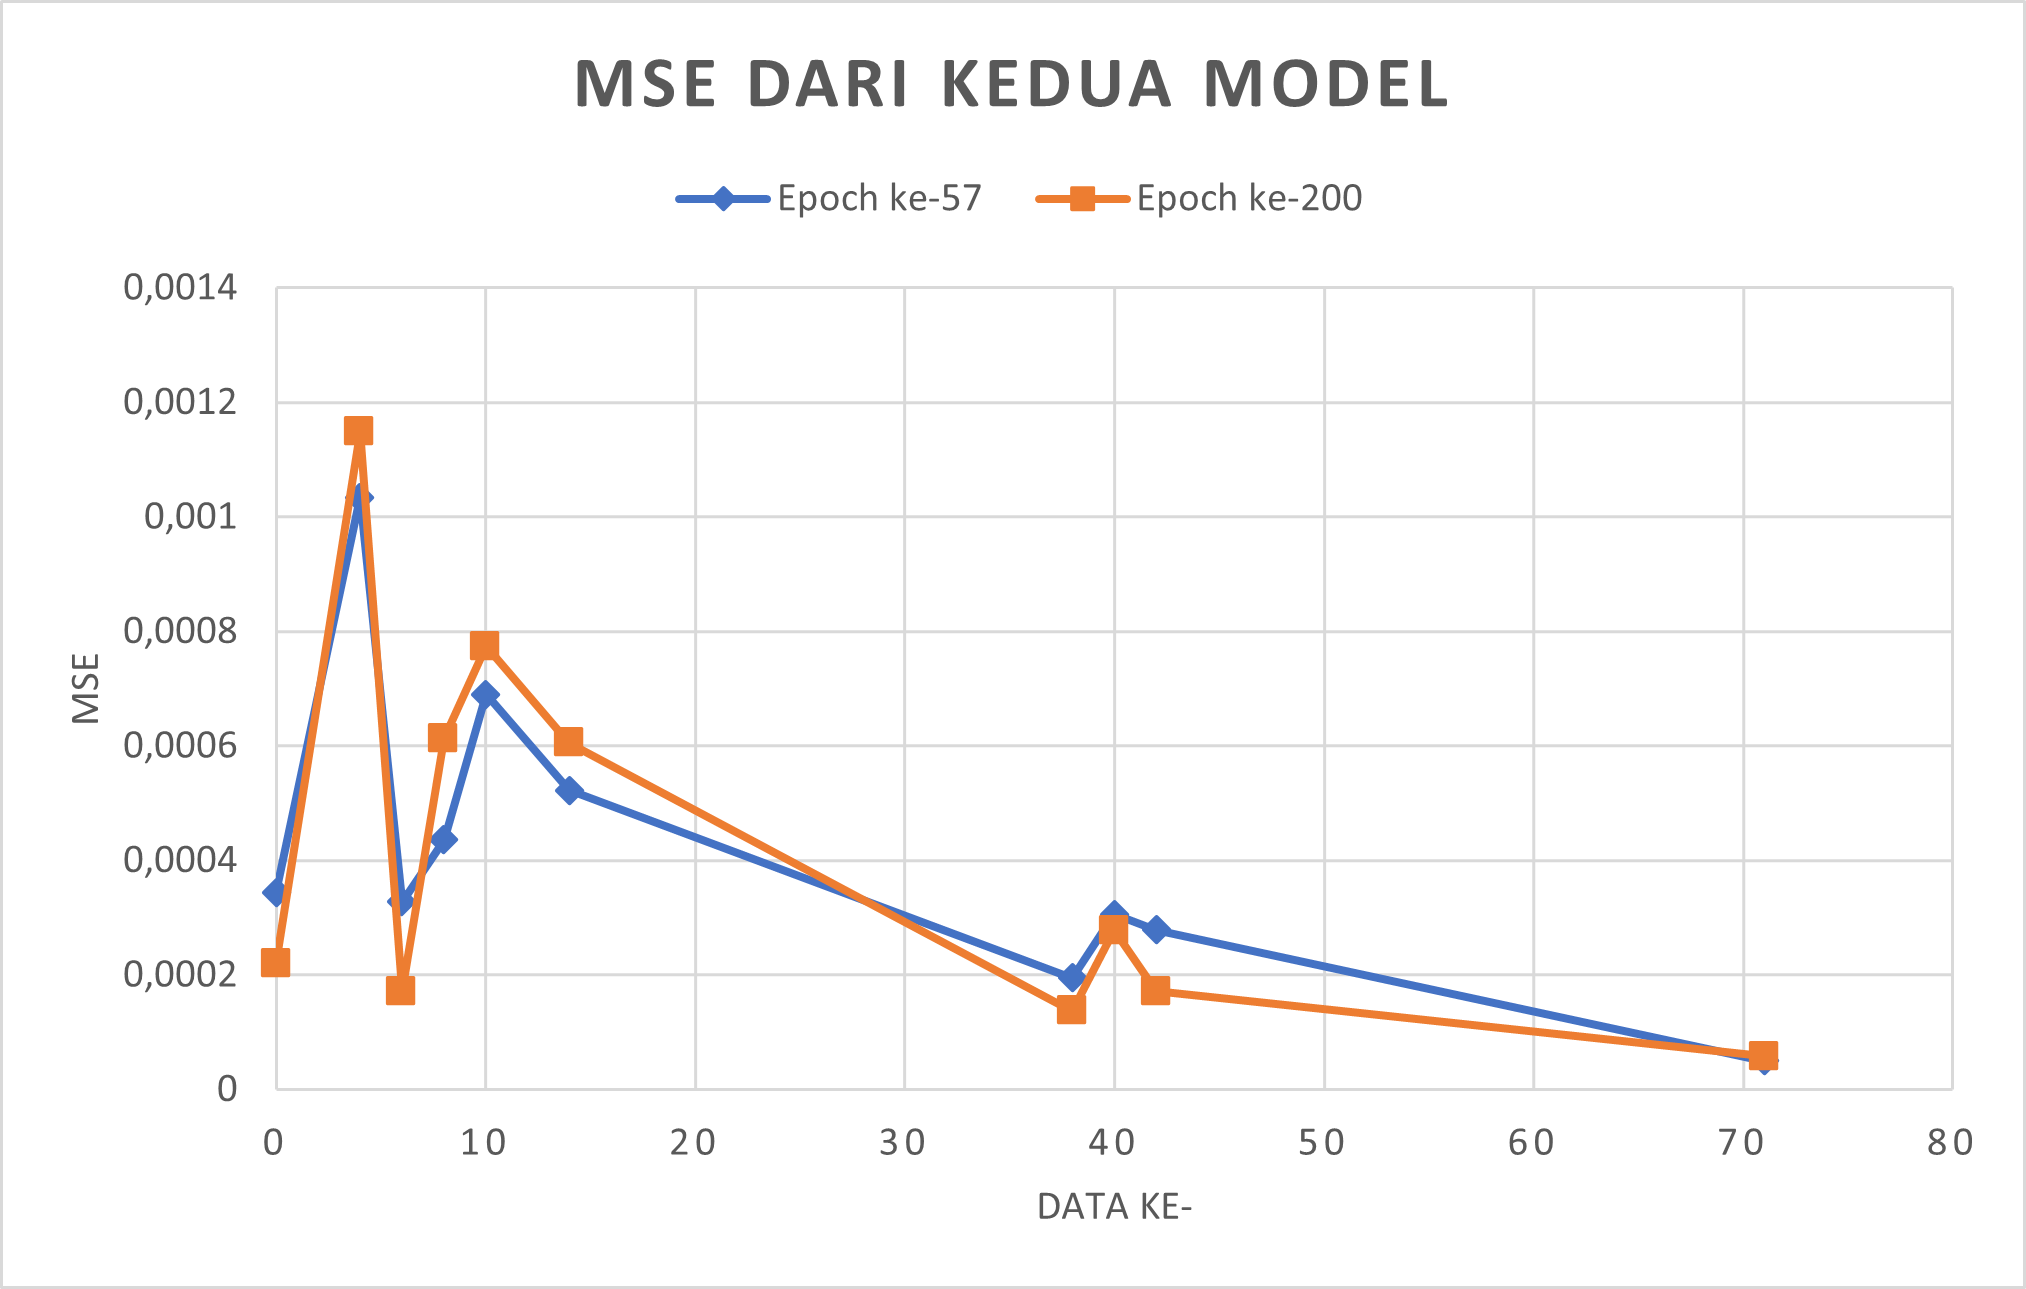
\includegraphics[width=12cm]{gambar/mse dari dua model.png}
%     \caption{MSE dari dua model dari 10 medan yang dihitung}
%     \label{mse2model}
% \end{figure}
%
% Akhirnya, dari hasil yang didapat, tetap harus dicatat bahwa metode yang diajukan tidak dapat dipandang sebagai pengganti metode numerik klasik dalam pemecahan permasalahan PDE. Metode tersebut sudah sangat matang dan mapan setelah penggunaan oleh berbagai teknisi dan ilmuwan selama lebih dari 50 tahun dan telah teruji berbagai standar ketahanan dan efisiensi komputasi yang disyaratkan \citep{DBLP:journals/corr/abs-1711-10561}.
%
% Penulis pribadi berpendapat bahwa hasil dari perhitungan metode CNN ini belum dapat diguankan sebagai pengganti murni perhitungan PDE. Namun sangat bisa sebagai tebakan awal dalam perhitungan iteratif seperti Gauss-Seidel yang harapannya berfungsi sebagai akselerator dalam konvergensi.
